\thispagestyle{toancuabinone}
\pagestyle{toancuabi}
\everymath{\color{toancuabi}}
%\blfootnote{$^1$\color{toancuabi}Đại học Thăng Long.}
\graphicspath{{../toancuabi/pic/}}
\begingroup
\AddToShipoutPicture*{\put(0,616){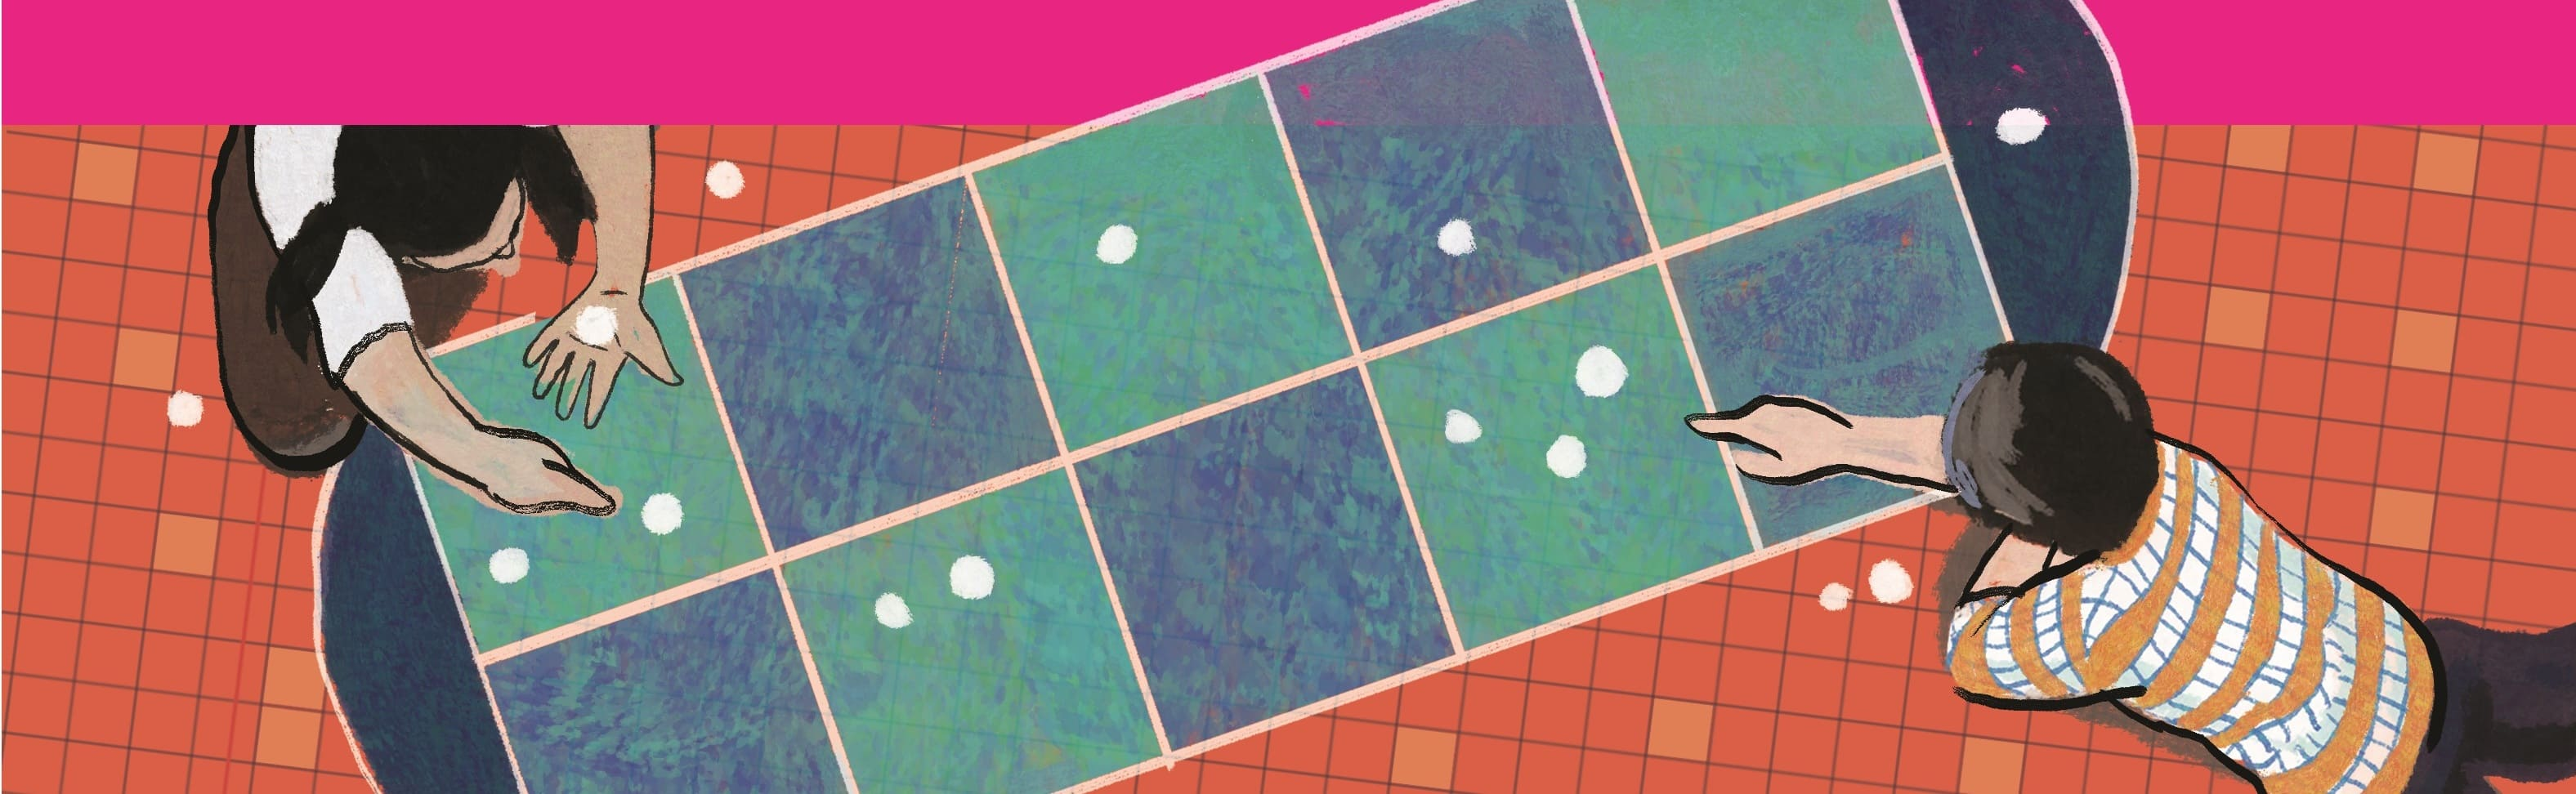
\includegraphics[width=19.3cm]{../bannertoancuabi}}}  
\AddToShipoutPicture*{\put(40,550){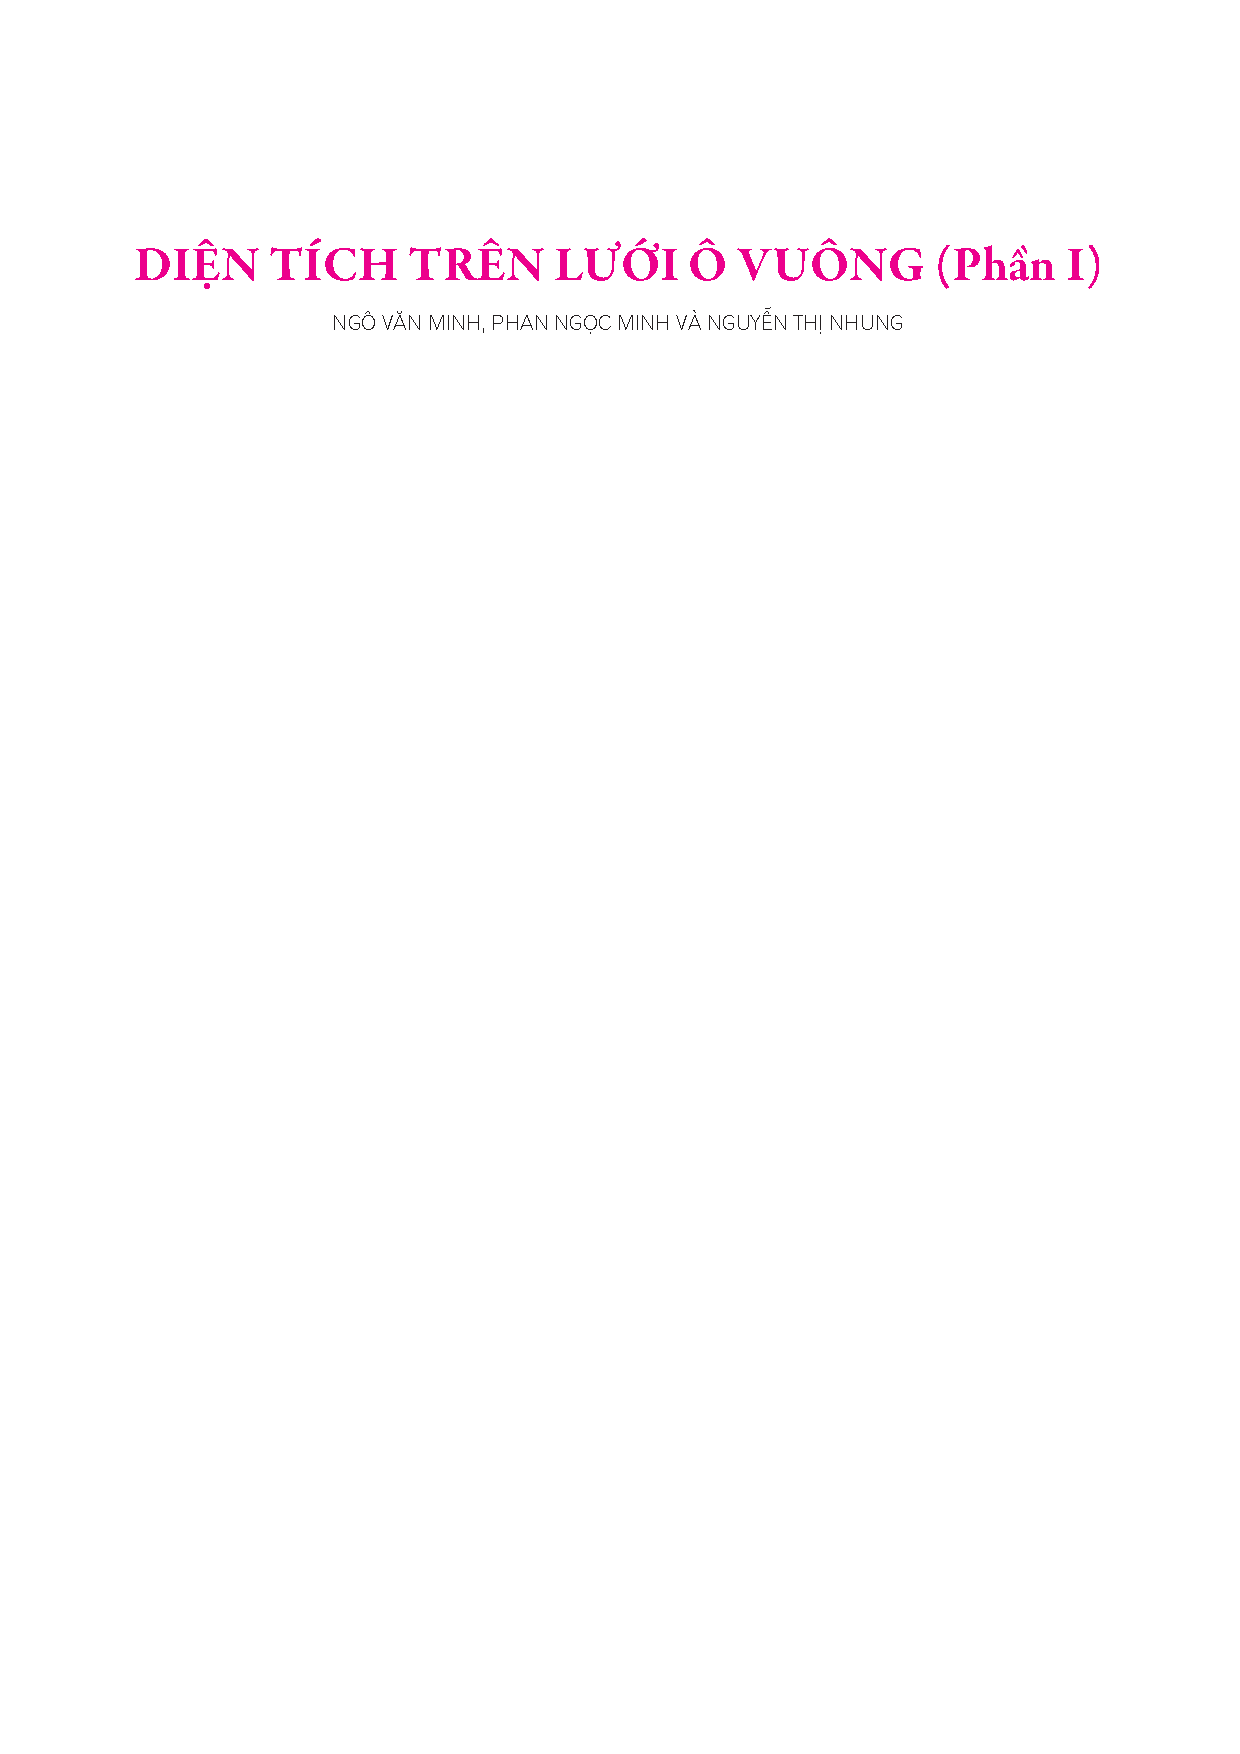
\includegraphics[scale=1]{../tieude1.pdf}}} 
\centering
\endgroup
\vspace*{155pt}

%\begin{multicols}{2}
%	Tính diện tích của một hình là một chủ đề hay và có nhiều điều thú vị của các bạn nhỏ cuối cấp $1$. Chủ đề này cũng được các thầy cô trong Câu lạc bộ Unicorn Math Circle (UMC) giảng dạy trong nhiều buổi với sự tham gia hào hứng của các bạn học và có nhiều cách giải độc đáo đã được đưa ra. Chúng ta cùng bắt đầu với một dạng tính diện tích trong những bài giảng của các thầy cô -- Tính diện tích hình trên lưới ô vuông. Với cách tính được trình bày trong bài viết này, các bạn nhỏ chưa học đến những công thức tính diện tích vẫn có thể tính được diện tích của nhiều kiểu hình khác nhau nhé, vì chúng ta chỉ dựa vào các ô vuông trên lưới thôi. Hơn thế nữa, dựa vào lưới ô vuông các em còn được khám phá những định lý nổi tiếng như Định lý Pythagoras, Định lý Pick và những tính chất hay khác của Toán học.
%	\vskip 0.1cm
%	$\pmb{1.}$ \textbf{\color{toancuabi}Diện tích của những hình cơ bản}
%	\begin{figure}[H]
	%			\centering
	%			\vspace*{-5pt}
	%			\captionsetup{labelformat= empty, justification=centering}
	%			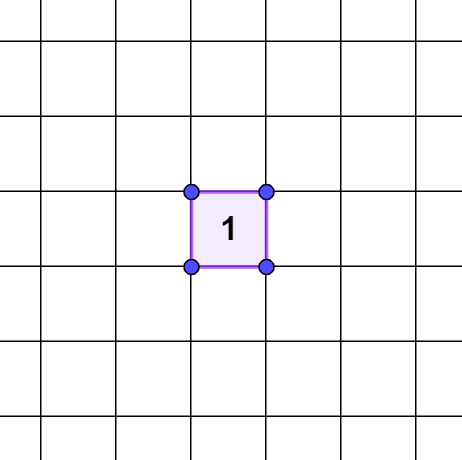
\includegraphics[width=0.45\linewidth]{1}
	%			\caption{\small\textit{\color{toancuabi}Hình $1$.}}
	%			\vspace*{-10pt}
	%		\end{figure}
%	Như nhiều bạn đã biết, lưới ô vuông gồm các đường thẳng song song cách đều nhau theo cả chiều ngang cũng như chiều dọc và tạo thành những hình vuông mà ta quy ước là chiếm $1$ đơn vị diện tích. Hình vuông đơn vị này là cơ sở để chúng ta tính diện tích của các hình tạo ra trên lưới trong các phần dưới đây.
%	\vskip 0.1cm
%	Trước hết ta bắt đầu với việc tìm diện tích của những hình rất đơn giản nhưng đóng vai trò quan trọng trong việc tính toán diện tích các hình ở các ví dụ sau.
%	\vskip 0.1cm
%	Hình cơ bản đầu tiên cần tính diện tích là hình vuông và hình chữ nhật có các cạnh nằm trên các đường thẳng của lưới.
%	\vskip 0.1cm
%	\textbf{\color{toancuabi}Ví dụ} $\pmb{1.}$ Tính diện tích của hai hình được tô đậm trong lưới ô vuông dưới đây.  
%	\begin{figure}[H]
	%		\centering
	%		\vspace*{-10pt}
	%		\captionsetup{labelformat= empty, justification=centering}
	%		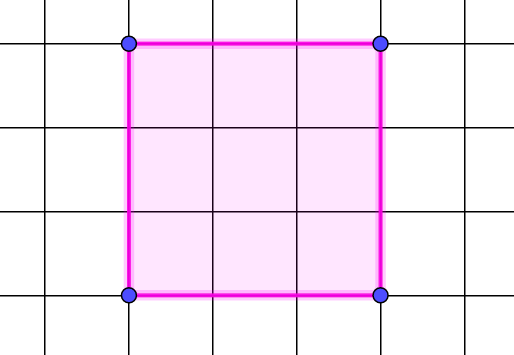
\includegraphics[width=0.4\linewidth]{2}
	%		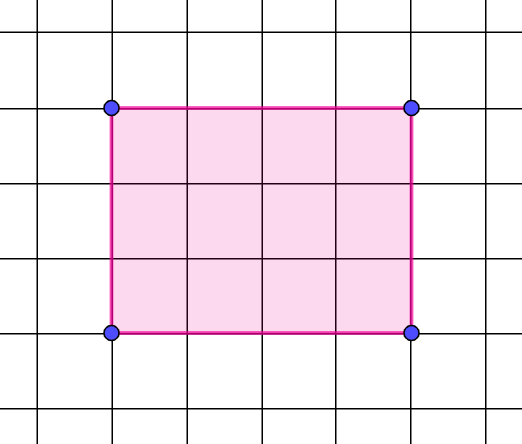
\includegraphics[width=0.45\linewidth]{3}
	%		\caption{\small\textit{\color{toancuabi}Hình $2$ \hspace*{40pt}Hình $3$.}}
	%		\vspace*{-15pt}
	%	\end{figure}
%	\textit{Lời giải.} Bằng cách đếm trực tiếp, ta thấy
%	\vskip 0.1cm
%	-- Hình $A$ có tổng cộng $9$ ô vuông nên có diện tích là $9$ đơn vị;
%	\vskip 0.1cm
%	-- Hình $B$ có tổng cộng $12$ ô vuông nên có diện tích phần hình bằng $12$ đơn vị.
%	\vskip 0.1cm
%	Các bạn mà học công thức tính diện tích hình vuông và hình chữ nhật rồi thì có thể nhận thấy ngay kết quả trên có thể tính được bằng cách sau.
%	\vskip 0.1cm
%	-- Cạnh của hình vuông là $3$ đơn vị nên diện tích là: $3 \times  3 = 9$ đơn vị;
%	\vskip 0.1cm
%	-- Hình chữ nhật chiều dài và chiều rộng tương ứng là $4$ và $3$ đơn vị nên có diện tích là: $4 \times  3 = 12$ đơn vị.
%	\vskip 0.1cm
%	Chúng ta tiếp tục với một hình cơ bản nữa là tam giác có hai cạnh trùng với hai đường dọc và ngang của lưới ô vuông.
%	\vskip 0.1cm
%	\textbf{\color{toancuabi}Ví dụ} $\pmb{2.}$ Tính diện tích tam giác được tô đậm trong hình dưới đây.
%	\begin{figure}[H]
	%		\centering
	%		\vspace*{-5pt}
	%		\captionsetup{labelformat= empty, justification=centering}
	%		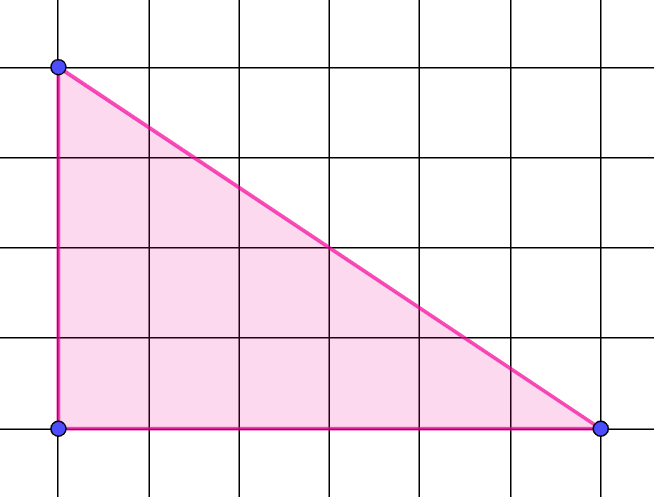
\includegraphics[width=0.5\linewidth]{4}
	%		\caption{\small\textit{\color{toancuabi}Hình $4$.}}
	%		\vspace*{-15pt}
	%	\end{figure}
%	\textit{Lời giải.} Ở ví dụ này, các bạn nhỏ quan sát một chút thì sẽ thấy ngay diện tích của tam giác đã cho bằng một nửa hình chữ nhật màu cỡ $6\times 4$ được tô màu xanh dương dưới đây.
%	\begin{figure}[H]
	%		\centering
	%		\vspace*{-5pt}
	%		\captionsetup{labelformat= empty, justification=centering}
	%		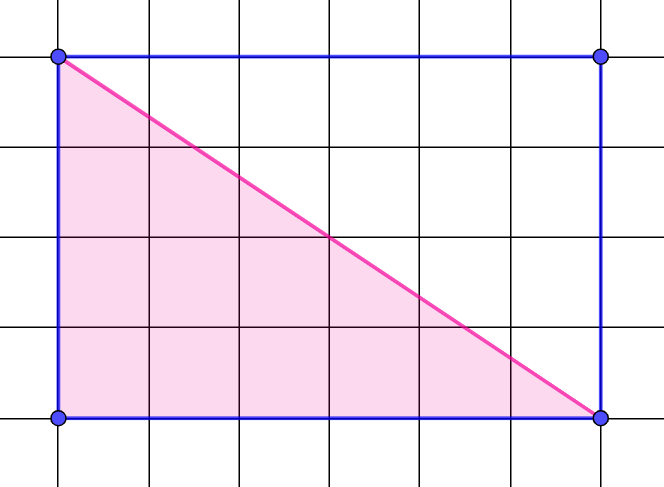
\includegraphics[width=0.5\linewidth]{5}
	%		\caption{\small\textit{\color{toancuabi}Hình $5$.}}
	%		\vspace*{-15pt}
	%	\end{figure}
%	Do diện tích hình chữ nhật được tạo bởi $24$ ô vuông nên diện tích hình tam giác bằng $\dfrac{24}{2}=12$ (đơn vị diện tích).
%	\vskip 0.1cm
%	Ngoài ra, nếu bạn nhỏ nào đã biết công thức tính diện tích tam giác thì hình trong Ví dụ $2$ là tam giác vuông với $2$ cạnh góc vuông là $6$ và $4$ đơn vị. Do đó diện tích của tam giác là $\dfrac{1}{2}\times 6\times 4 = 12$ đơn vị.
%	\vskip 0.1cm
%	Hai ví dụ trên cho ta một cái nhìn trực quan về bài toán tính diện tích trên lưới ô vuông, ta chỉ đơn giản dùng cách đếm đơn thuần số ô vuông trên lưới. Trong các bài toán sau, có thể có nhiều cách giải khác nhau nhưng bài viết đưa ra cách giải mà chỉ dựa vào những hình cơ bản đã biết cách tính diện tích trong Ví dụ $1$ và Ví dụ $2$.
%	\vskip 0.1cm
%	$\pmb{2.}$ \textbf{\color{toancuabi}Diện tích hình chia thành những hình cơ bản}
%	\vskip 0.1cm
%	Chúng ta lại tiếp tục với tính diện tích của tam giác nhé. Lần này là tam giác chỉ có một cạnh trùng với đường dọc--ngang của lưới và nhận thấy ta không thể áp dụng luôn cách tính như trong Ví dụ $2$. Tuy nhiên bằng cách chia tam giác đã cho thành các tam giác nhỏ có hai cạnh trùng với những đường thẳng của lưới, ta hoàn toàn có thể áp dụng cách tính diện tích tam giác như trong tình huống trên.
%	\vskip 0.1cm
%	\textbf{\color{toancuabi}Ví dụ} $\pmb{3.}$ Tính diện tích tam giác được tô đậm trong hình cho ở dưới đây.
%	\begin{figure}[H]
	%		\centering
	%		\vspace*{-5pt}
	%		\captionsetup{labelformat= empty, justification=centering}
	%		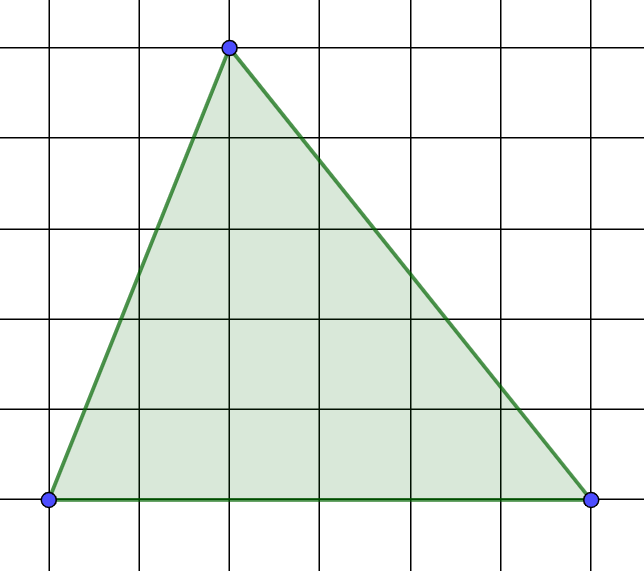
\includegraphics[width=0.5\linewidth]{6}
	%		\caption{\small\textit{\color{toancuabi}Hình $6$.}}
	%		\vspace*{-10pt}
	%	\end{figure}
%	\textit{Lời giải.} Ta chia hình tam giác lớn thành hai hình tam giác $(1)$ và $(2)$.
%	\begin{figure}[H]
	%		\centering
	%		\vspace*{-5pt}
	%		\captionsetup{labelformat= empty, justification=centering}
	%		
\includegraphics[width=0.5\linewidth]{7}
	%		\caption{\small\textit{\color{toancuabi}Hình $7$.}}
	%		\vspace*{-10pt}
	%	\end{figure}
%	Sau đó tính diện tích từng tam giác, tương tự như trong Ví dụ $2$.
%	\begin{figure}[H]
	%		\centering
	%		\vspace*{-5pt}
	%		\captionsetup{labelformat= empty, justification=centering}
	%		
\includegraphics[width=0.5\linewidth]{8}
	%		\caption{\small\textit{\color{toancuabi}Hình $8$.}}
	%		\vspace*{-5pt}
	%	\end{figure}
%	Hình tam giác $(1)$ có diện tích bằng một nửa hình chữ nhật bên trái nên có diện tích là: $\dfrac{10}{2}=5$ (đơn vị diện tích).
%	\vskip 0.1cm
%	Hình tam giác $(2)$ có diện tích bằng một nửa hình chữ nhật bên phải và do đó có diện tích là: $\dfrac{20}{2}=10$ (đơn vị diện tích).
%	\vskip 0.1cm
%	Suy ra hình cần tính có diện tích bằng $5+10=15$ (đơn vị diện tích). 
%	\vskip 0.1cm
%	Tính diện tích bằng cách chia hình thành những hình nhỏ hơn không chỉ dừng lại ở việc tính toán những dạng hình học quen thuộc như hình tam giác, hình chữ nhật, ... mà còn có thể áp dụng cho rất kiểu hình khác nhau. Chẳng hạn như hình ``chú mèo`` ngộ nghĩnh dưới đây.  
%	\vskip 0.1cm
%	\textbf{\color{toancuabi}Ví dụ} $\pmb{4.}$ Tính diện tích ``chú mèo`` được cho bởi phần tô đậm trong hình sau.
%	\begin{figure}[H]
	%		\centering
	%		\vspace*{-5pt}
	%		\captionsetup{labelformat= empty, justification=centering}
	%		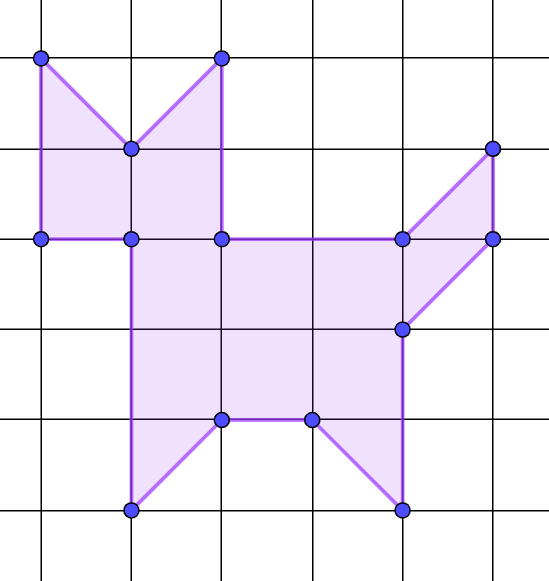
\includegraphics[width=0.45\linewidth]{9}
	%		\caption{\small\textit{\color{toancuabi}Hình $9$.}}
	%		\vspace*{-10pt}
	%	\end{figure}
%	\textit{Lời giải.} Ở hình trên có những tam giác nửa, tức là tam giác có diện tích bằng một nửa hình vuông đơn vị và có diện tích là $\dfrac{1}{2}$ đơn vị diện tích. Ta đếm có tổng cộng $8$ hình vuông và $6$ hình tam giác nửa ($2$ tai, $2$ chân và cái đuôi). Vì thế ``chú mèo`` có diện tích bằng $8+\dfrac{1}{2}\times 6=11$ đơn vị diện tích.
%	\vskip 0.1cm
%	Một chú ngựa xinh xắn cần tính diện tích cho các em luyện tập thêm nhé.
%	\vskip 0.1cm
%	\textbf{\color{toancuabi}Bài tập} $\pmb{1.}$ Tìm diện tích ``chú ngựa`` trong hình sau.
%	\begin{figure}[H]
	%		\centering
	%		\vspace*{5pt}
	%		\captionsetup{labelformat= empty, justification=centering}
	%		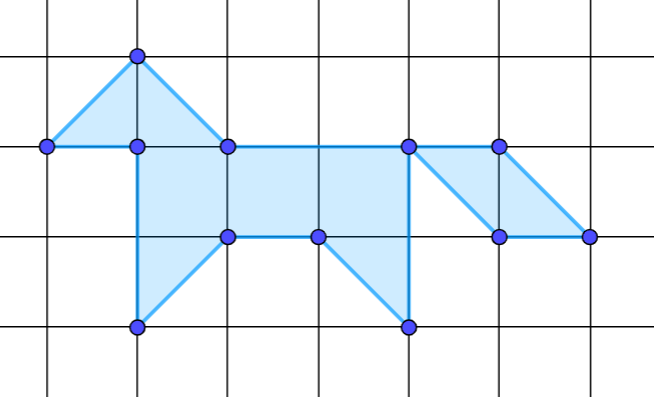
\includegraphics[width=0.45\linewidth]{10}
	%		\caption{\small\textit{\color{toancuabi}Hình $10$.}}
	%		\vspace*{-10pt}
	%	\end{figure}
%	$\pmb{3.}$ \textbf{\color{toancuabi}Diện tích hình tính theo phần bù}
%	\vskip 0.1cm
%	Diện tích cần tính dưới đây tiếp tục là một tam giác, nhưng lần này là một tam giác tùy ý, không có cạnh nào trùng với những đường thẳng của lưới. 
%	\vskip 0.1cm
%	\textbf{\color{toancuabi}Ví dụ} $\pmb{5.}$ Tính diện tích của hình được tô đậm sau đây.
%	\begin{figure}[H]
	%		\centering
	%		\vspace*{-5pt}
	%		\captionsetup{labelformat= empty, justification=centering}
	%		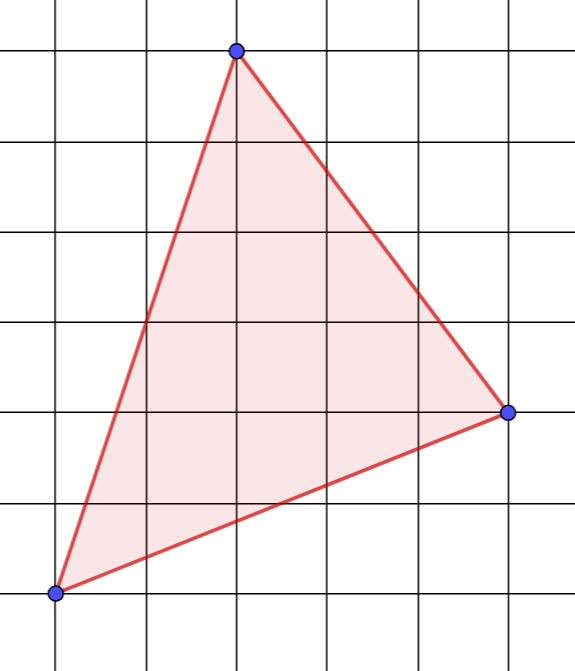
\includegraphics[width=0.42\linewidth]{11}
	%		\caption{\small\textit{\color{toancuabi}Hình $11$.}}
	%		\vspace*{-10pt}
	%	\end{figure}
%	\textit{Lời giải.} Rõ ràng với tam giác này, việc tính trực tiếp phần bên trong là khó khăn. Tuy nhiên phần bù của tam giác trong hình chữ nhật bao quanh nó lại là những tam giác như trong Ví dụ $2$ nên ta hoàn toàn có thể tính được ngay.
%	\begin{figure}[H]
	%		\centering
	%		\vspace*{-5pt}
	%		\captionsetup{labelformat= empty, justification=centering}
	%		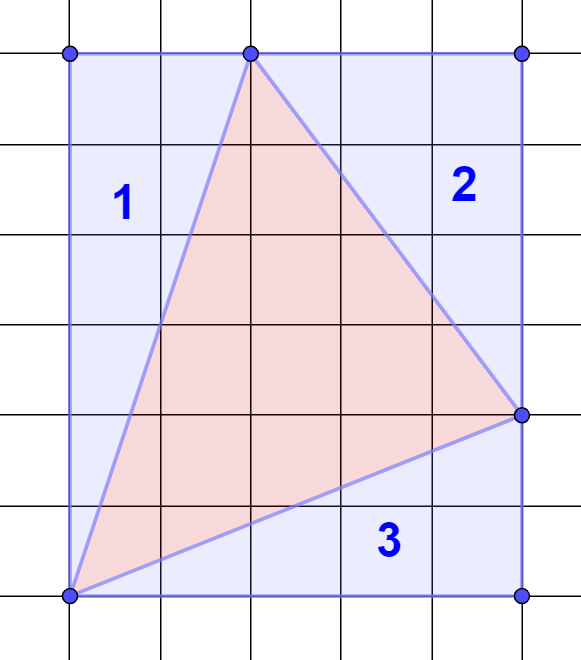
\includegraphics[width=0.42\linewidth]{12}
	%		\caption{\small\textit{\color{toancuabi}Hình $12$.}}
	%		\vspace*{-10pt}
	%	\end{figure}
%	Lần lượt gọi ba tam giác phần bù được tô xanh là $(1)$, $(2)$ và $(3)$. Ta thấy:
%	\vskip 0.1cm
%	-- Hình $(1)$ có diện tích bằng nửa hình chữ nhật cỡ $6\times 2$, nên có diện tích bằng $6$.
%	\vskip 0.1cm
%	-- Hình $(2)$ có diện tích bằng nửa hình chữ nhật cỡ $4\times 3$, nên có diện tích bằng $6$.
%	\vskip 0.1cm
%	-- Hình $(3)$ có diện tích bằng nửa hình chữ nhật cỡ $5\times 2$, nên có diện tích bằng $5$.
%	\vskip 0.1cm
%	Vì phần bù được tạo thành bởi ba tam giác vuông $(1)$, $(2)$ và $(3)$ nên diện tích của chúng bằng $6+6+5=17$. Suy ra diện tích tam giác được tô đậm bằng $30-17=13$ (đơn vị diện tích).
%	\vskip 0.1cm
%	Để rèn luyện thêm cách tính diện tích dựa trên phần bù, chúng ta cùng làm tiếp ví dụ sau.  
%	\vskip 0.1cm
%	\textbf{\color{toancuabi}Ví dụ} $\pmb{6.}$ Tính diện tích phần hình được tô đậm dưới đây.
%	\begin{figure}[H]
	%		\centering
	%		\vspace*{-5pt}
	%		\captionsetup{labelformat= empty, justification=centering}
	%		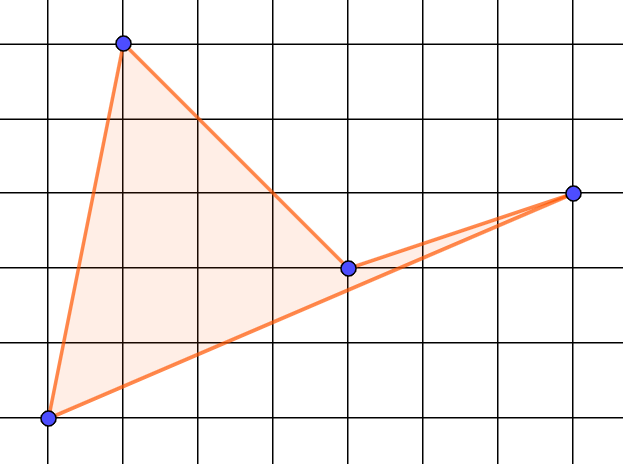
\includegraphics[width=0.5\linewidth]{13}
	%		\caption{\small\textit{\color{toancuabi}Hình $13$.}}
	%		\vspace*{-10pt}
	%	\end{figure}
%	\textit{Lời giải.} Trong ví dụ này, ta tiếp tục tính diện tích theo phần bù và chia phần bù của hình đã cho thành các hình quen thuộc đã biết cách tính diện tích. Mỗi bạn nhỏ có thể chọn những cách chia khác nhau, chẳng hạn ta có thể chia đơn giản như sau: 
%	\begin{figure}[H]
	%		\centering
	%		\vspace*{-5pt}
	%		\captionsetup{labelformat= empty, justification=centering}
	%		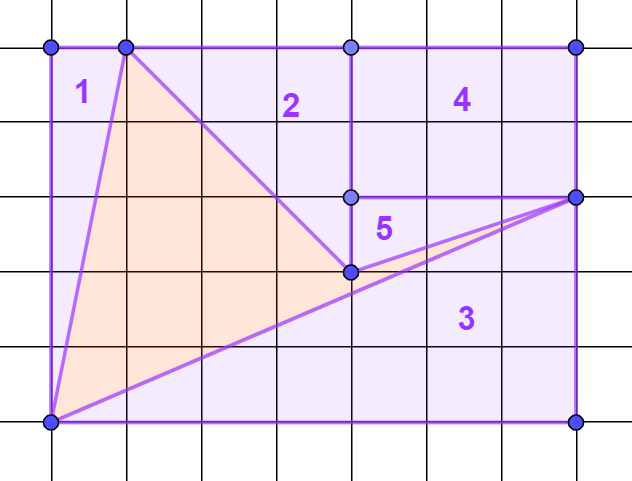
\includegraphics[width=0.5\linewidth]{14}
	%		\caption{\small\textit{\color{toancuabi}Hình $14$.}}
	%		\vspace*{-10pt}
	%	\end{figure}
%	Phần bù của hình đã cho được chia thành năm hình $(1)$, $(2)$, $(3)$, $(4)$ và $(5)$. Khi đó
%	\vskip 0.1cm
%	-- Hình tam giác $(1)$ có diện tích bằng $\dfrac{1}{2}\times 5=2{,}5$ (đơn vị diện tích)
%	\vskip 0.1cm
%	-- Hình tam giác $(2)$ có diện tích bằng $\dfrac{1}{2}\times 9=4{,}5$ (đơn vị diện tích)
%	\vskip 0.1cm
%	-- Hình tam giác $(3)$ có diện tích bằng $\dfrac{1}{2}\times 21=10{,}5$ (đơn vị diện tích)
%	\vskip 0.1cm
%	-- Hình chữ nhật $(4)$ có diện tích bằng $6$ (đơn vị diện tích)
%	\vskip 0.1cm
%	-- Hình tam giác $(5)$ có diện tích bằng $\dfrac{1}{2}\times 3=1{,}5$ (đơn vị diện tích)
%	\vskip 0.1cm
%	Vậy tổng diện tích của chúng bằng $2{,}5+4{,}5+10{,}5+6+1{,}5 =25$. Suy ra diện tích hình tam giác tô đậm bằng $7\times 7-25=24$ (đơn vị diện tích). 
%	\vskip 0.1cm
%	Việc tính theo phần bù chỉ hiệu quả khi phần bù được cấu tạo bởi những hình cơ bản như hình chữ nhật, hình tam giác như trong hai ví dụ đầu tiên. Vì thế các bạn nhỏ cần chia thật khéo, sao cho mọi hình đều có dạng quen thuộc nhé!  
%	\vskip 0.1cm
%	Cô nàng ``bướm" xinh đẹp dưới đây để thử tài chia hình của các bạn nhỏ.
%	\vskip 0.1cm
%	\textbf{\color{toancuabi}Bài tập} $\pmb{2.}$ Tính diện tích phần được tô đậm trong hình sau.
%	\begin{figure}[H]
	%		\centering
	%		\vspace*{-5pt}
	%		\captionsetup{labelformat= empty, justification=centering}
	%		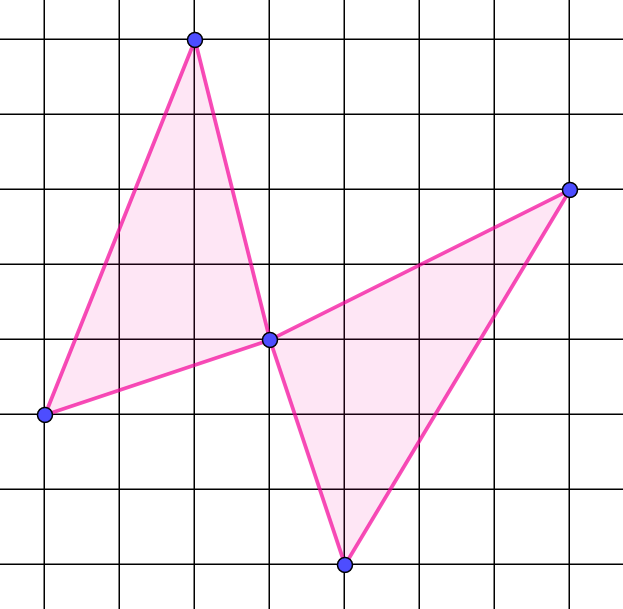
\includegraphics[width=0.5\linewidth]{15}
	%		\caption{\small\textit{\color{toancuabi}Hình $15$.}}
	%		\vspace*{-10pt}
	%	\end{figure}
%	Bây giờ chúng ra sẽ vận dụng cách tính diện tích được giới thiệu ở trên để làm một điều rất thú vị, đó là chứng minh một định lý rất quen thuộc trong Toán học: Định lý Pythagoras.
%	\vskip 0.1cm
%	$\pmb{4.}$ \textbf{\color{toancuabi}Diện tích và định lý Pythagoras}
%	\vskip 0.1cm
%	Hẳn nhiều bạn nhỏ đã biết về định lý Pythagoras rồi đúng không. Định lý Pythagoras phát biểu rằng: ``Trong một tam giác vuông, bình phương của cạnh huyền bằng tổng bình phương của hai cạnh góc vuông``, ở đây bình phương của số a, ký hiệu là $a^2$ là tích của $a$ nhân với $a$, $a^2=a\times a$.
%	\vskip 0.1cm
%	Giả sử tam giác vuông có hai cạnh góc vuông là $a$ và $b$, cạnh huyền là $c$. Khi đó, định lý Pythagoras cho ta đẳng thức: $a^2+b^2=c^2$. Trong bài viết này, ta xét $a$, $b$ và $c$ là các số tự nhiên khác không, tuy nhiên những lập luận dưới đây đúng cho tam giác vuông với các cạnh không cần là số tự nhiên các em nhé. 
%	\begin{figure}[H]
	%		\centering
	%		\vspace*{-5pt}
	%		\captionsetup{labelformat= empty, justification=centering}
	%		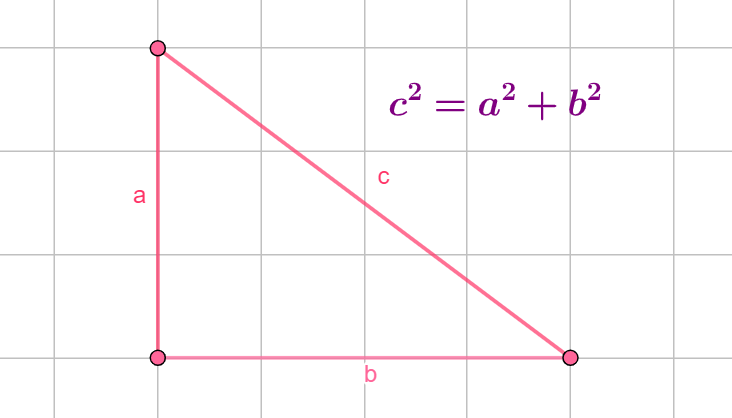
\includegraphics[width=0.5\linewidth]{16}
	%		\caption{\small\textit{\color{toancuabi}Hình $16$.}}
	%		\vspace*{-10pt}
	%	\end{figure}
%	Bây giờ chúng ta cùng xem chứng minh định lý Pythagoras dựa trên việc tính diện tích các hình thế nào.
%	\vskip 0.1cm
%	Trước hết nhận thấy rằng $a^2$, $b^2$ hay $c^2$ chính là diện tích của các hình vuông với cạnh tương ứng là $a$, $b$ hay $c$. Ở đây, chúng ta sẽ dựa trên việc tính diện tích của các hình này để suy ra định lý Pythagoras. 
%	\begin{figure}[H]
	%		\centering
	%		\vspace*{-5pt}
	%		\captionsetup{labelformat= empty, justification=centering}
	%		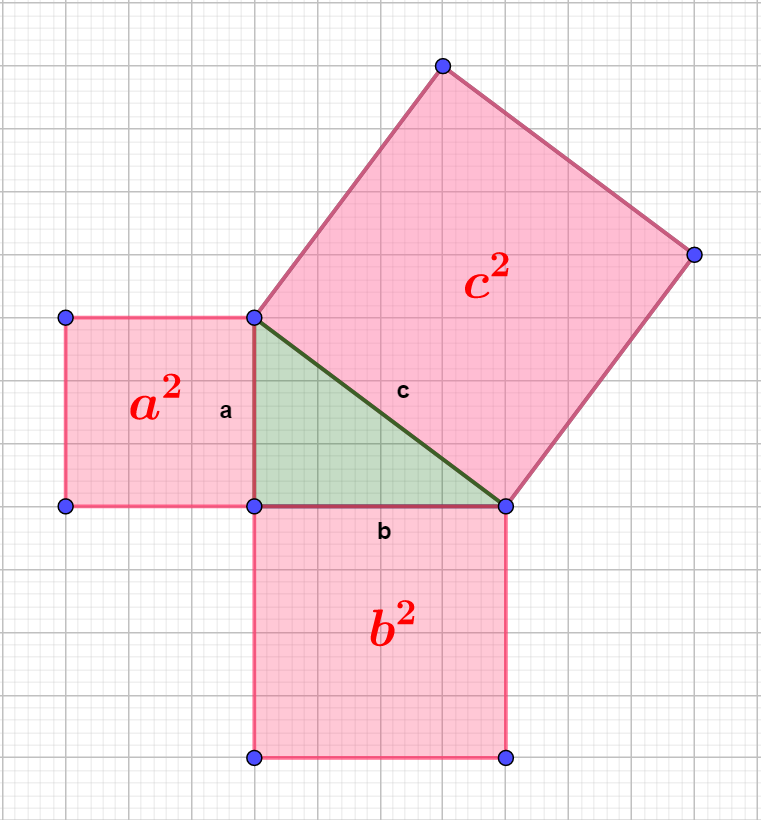
\includegraphics[width=0.5\linewidth]{17}
	%		\caption{\small\textit{\color{toancuabi}Hình $17$.}}
	%		\vspace*{-10pt}
	%	\end{figure}
%	Đầu tiên là ta tính diện tích của hình vuông cạnh $c$ được tô màu hồng trong Hình $19$. Diện tích của hình vuông này có thể được tính bằng cách lấy phần bù trong hình vuông bao quanh với cạnh là $a+b$. Các em có thể thấy ngay phần bù của hình vuông cần tính là $4$ tam giác vuông có diện tích bằng diện tích của tam giác vuông đã cho.
%	\begin{figure}[H]
	%		\centering
	%		\vspace*{-5pt}
	%		\captionsetup{labelformat= empty, justification=centering}
	%		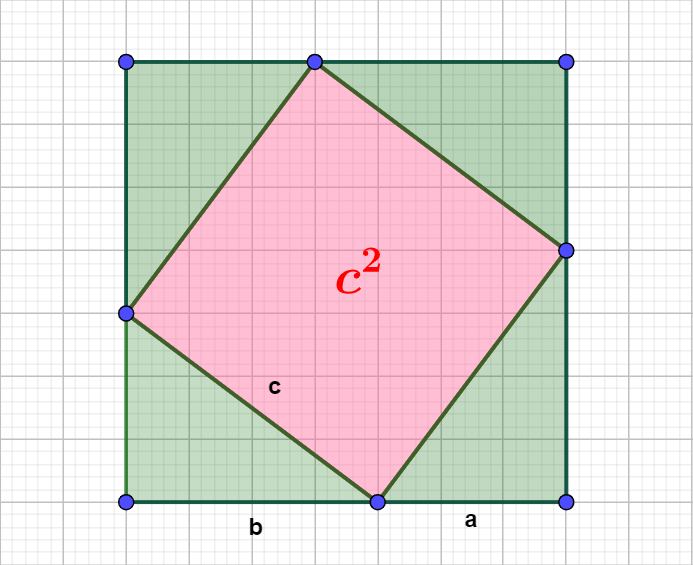
\includegraphics[width=0.5\linewidth]{18}
	%		\caption{\small\textit{\color{toancuabi}Hình $18$.}}
	%		\vspace*{-5pt}
	%	\end{figure}
%	Tiếp đến ta tính diện tích của hai hình vuông màu hồng có cạnh tương ứng là $b$ và $c$ trong Hình $20$. Phần bù của tổng diện tích hai tam giác này trong hình vuông bao quanh (cạnh là $a+b$) cũng là $4$ tam giác vuông có diện tích bằng tam giác đã cho.
%	\begin{figure}[H]
	%		\centering
	%		\vspace*{-5pt}
	%		\captionsetup{labelformat= empty, justification=centering}
	%		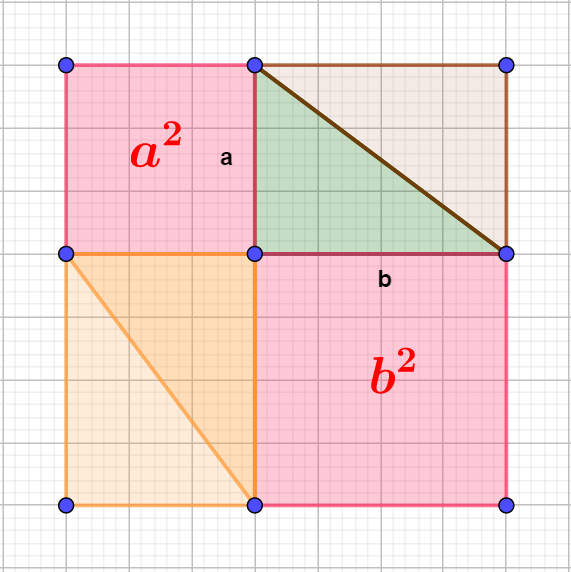
\includegraphics[width=0.48\linewidth]{19}
	%		\caption{\small\textit{\color{toancuabi}Hình $19$.}}
	%		\vspace*{-10pt}
	%	\end{figure}
%	Do hai hình vuông bao quanh đều có cạnh là $a+b$ nên có cùng diện tích. Từ đó ta có ngay: $a^2+b^2=c^2$ và chứng minh được định lý Pythagoras!
%	\begin{figure}[H]
	%		\centering
	%		\vspace*{-5pt}
	%		\captionsetup{labelformat= empty, justification=centering}
	%		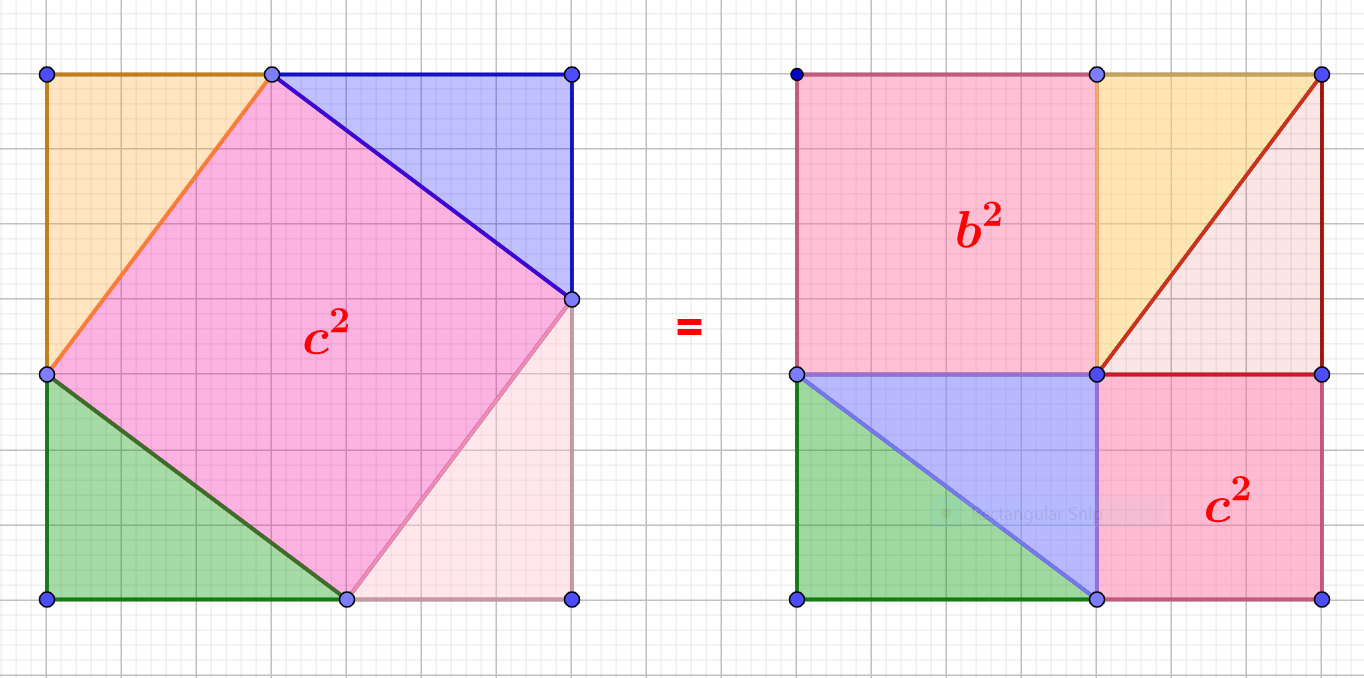
\includegraphics[width=1\linewidth]{20}
	%		\caption{\small\textit{\color{toancuabi}Hình $20$.}}
	%		\vspace*{-10pt}
	%	\end{figure}
%	Vậy là bằng cách tính diện tích của những hình cơ bản là hình vuông và tam giác vuông mà chúng ta đã chứng minh được một định lý rất nổi tiếng. Thật là kỳ diệu phải không các em!
%	\vskip 0.1cm
%	Trong phần đầu tiên của chủ đề này, chúng ta đã cùng nhau tìm hiểu những phương pháp thường được sử dụng khi tính diện tích của một hình trên lưới ô vuông. Những cách đưa ra dù rất đơn giản nhưng lại giúp ta làm được một điều rất hữu ích -- chứng mình được định lý Pythagoras. Chủ đề diện tích trên lưới ô vuông vẫn còn nhiều thú vị nữa các bạn nhỏ nhé, các em hãy đón đọc Phần $2$ của chủ đề trong số sau của Pi.	
%\end{multicols}
\newpage
\begingroup
\AddToShipoutPicture*{\put(140,678){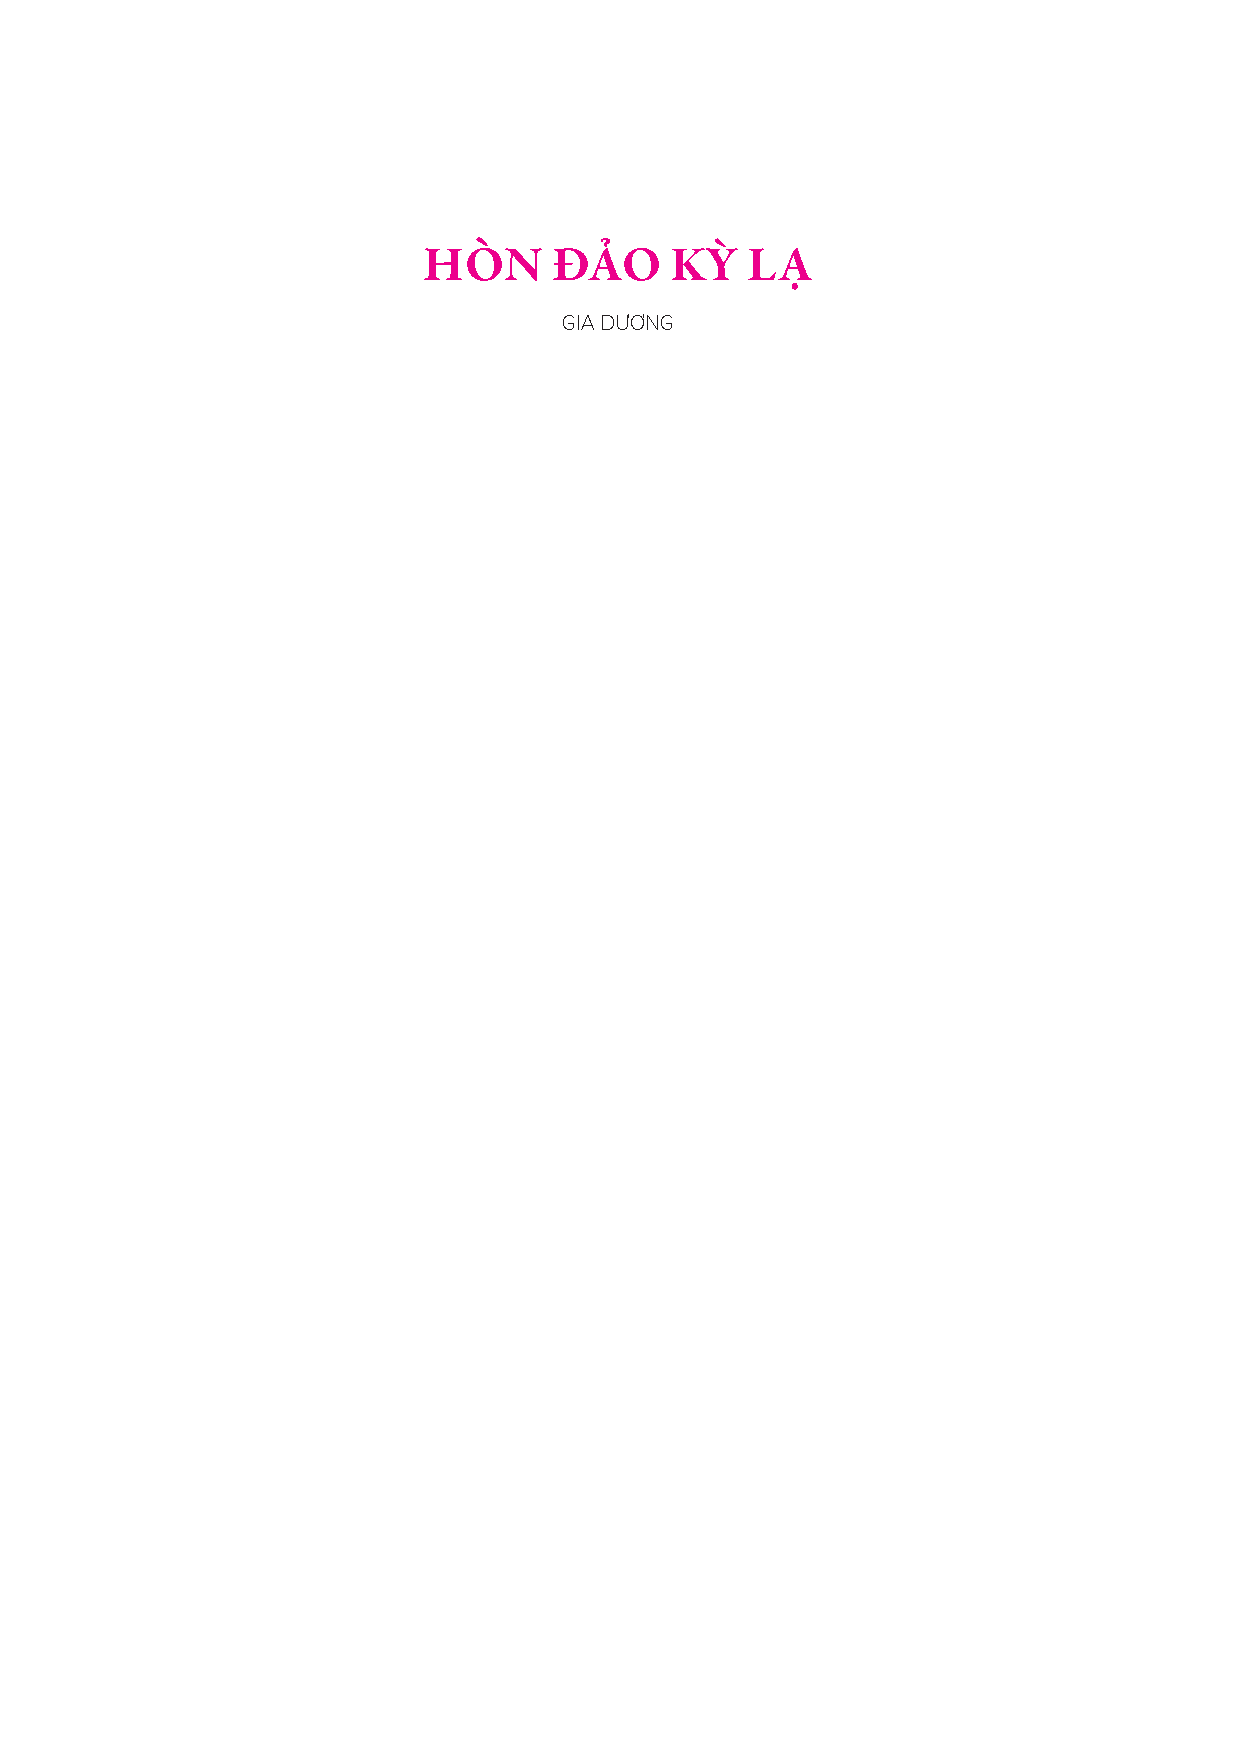
\includegraphics[scale=1]{../tieude.pdf}}} 
\centering
\endgroup
\vspace*{30pt}

\begin{multicols}{2}
	Thám tử Xuân Phong lại lên đường truy tìm tên trùm Cạ đang bị lệnh truy nã. Xuân Phong chỉ biết hắn ta đang lẩn quất tại một địa điểm tên là làng Đoài, còn đường đi tới đó thế nào thì không rõ. Cứ theo những người đi đường chỉ dẫn, Xuân Phong cuối cùng cũng đi tới một ngã ba, từ đó đường bỗng chia thành hai ngả, một ngả rẽ trái, một ngả rẽ phải, thật mung lung. Xuân Phong bỗng nhìn thấy một quán nước nhỏ bên vệ đường. Ông chủ quán bước ra đon đả mời Xuân Phong vào nghỉ chân, xơi nước cho đỡ mệt. Quán của ông này nổi tiếng cả vùng, Xuân Phong cũng đã từng nghe thấy nói tới ông chủ là một người vô cùng đặc biệt. Ông ta cứ một hôm lại nói dối, rồi lại nói thật ngày hôm sau, và cứ cách nhật như vậy -- hôm nói thật và hôm nói dối xen kẽ ngày. Xuân Phong có thể hỏi ông chủ quán đúng một câu hỏi để biết cách chọn đúng đường rẽ tới làng Đoài mà trùm Cạ đang trốn. Vậy Xuân Phong có thể hỏi ông ta câu hỏi nào để biết đường nào sẽ đi tới làng Đoài?
	\begin{figure}[H]
		\vspace*{-5pt}
		\centering
		\captionsetup{labelformat= empty, justification=centering}
		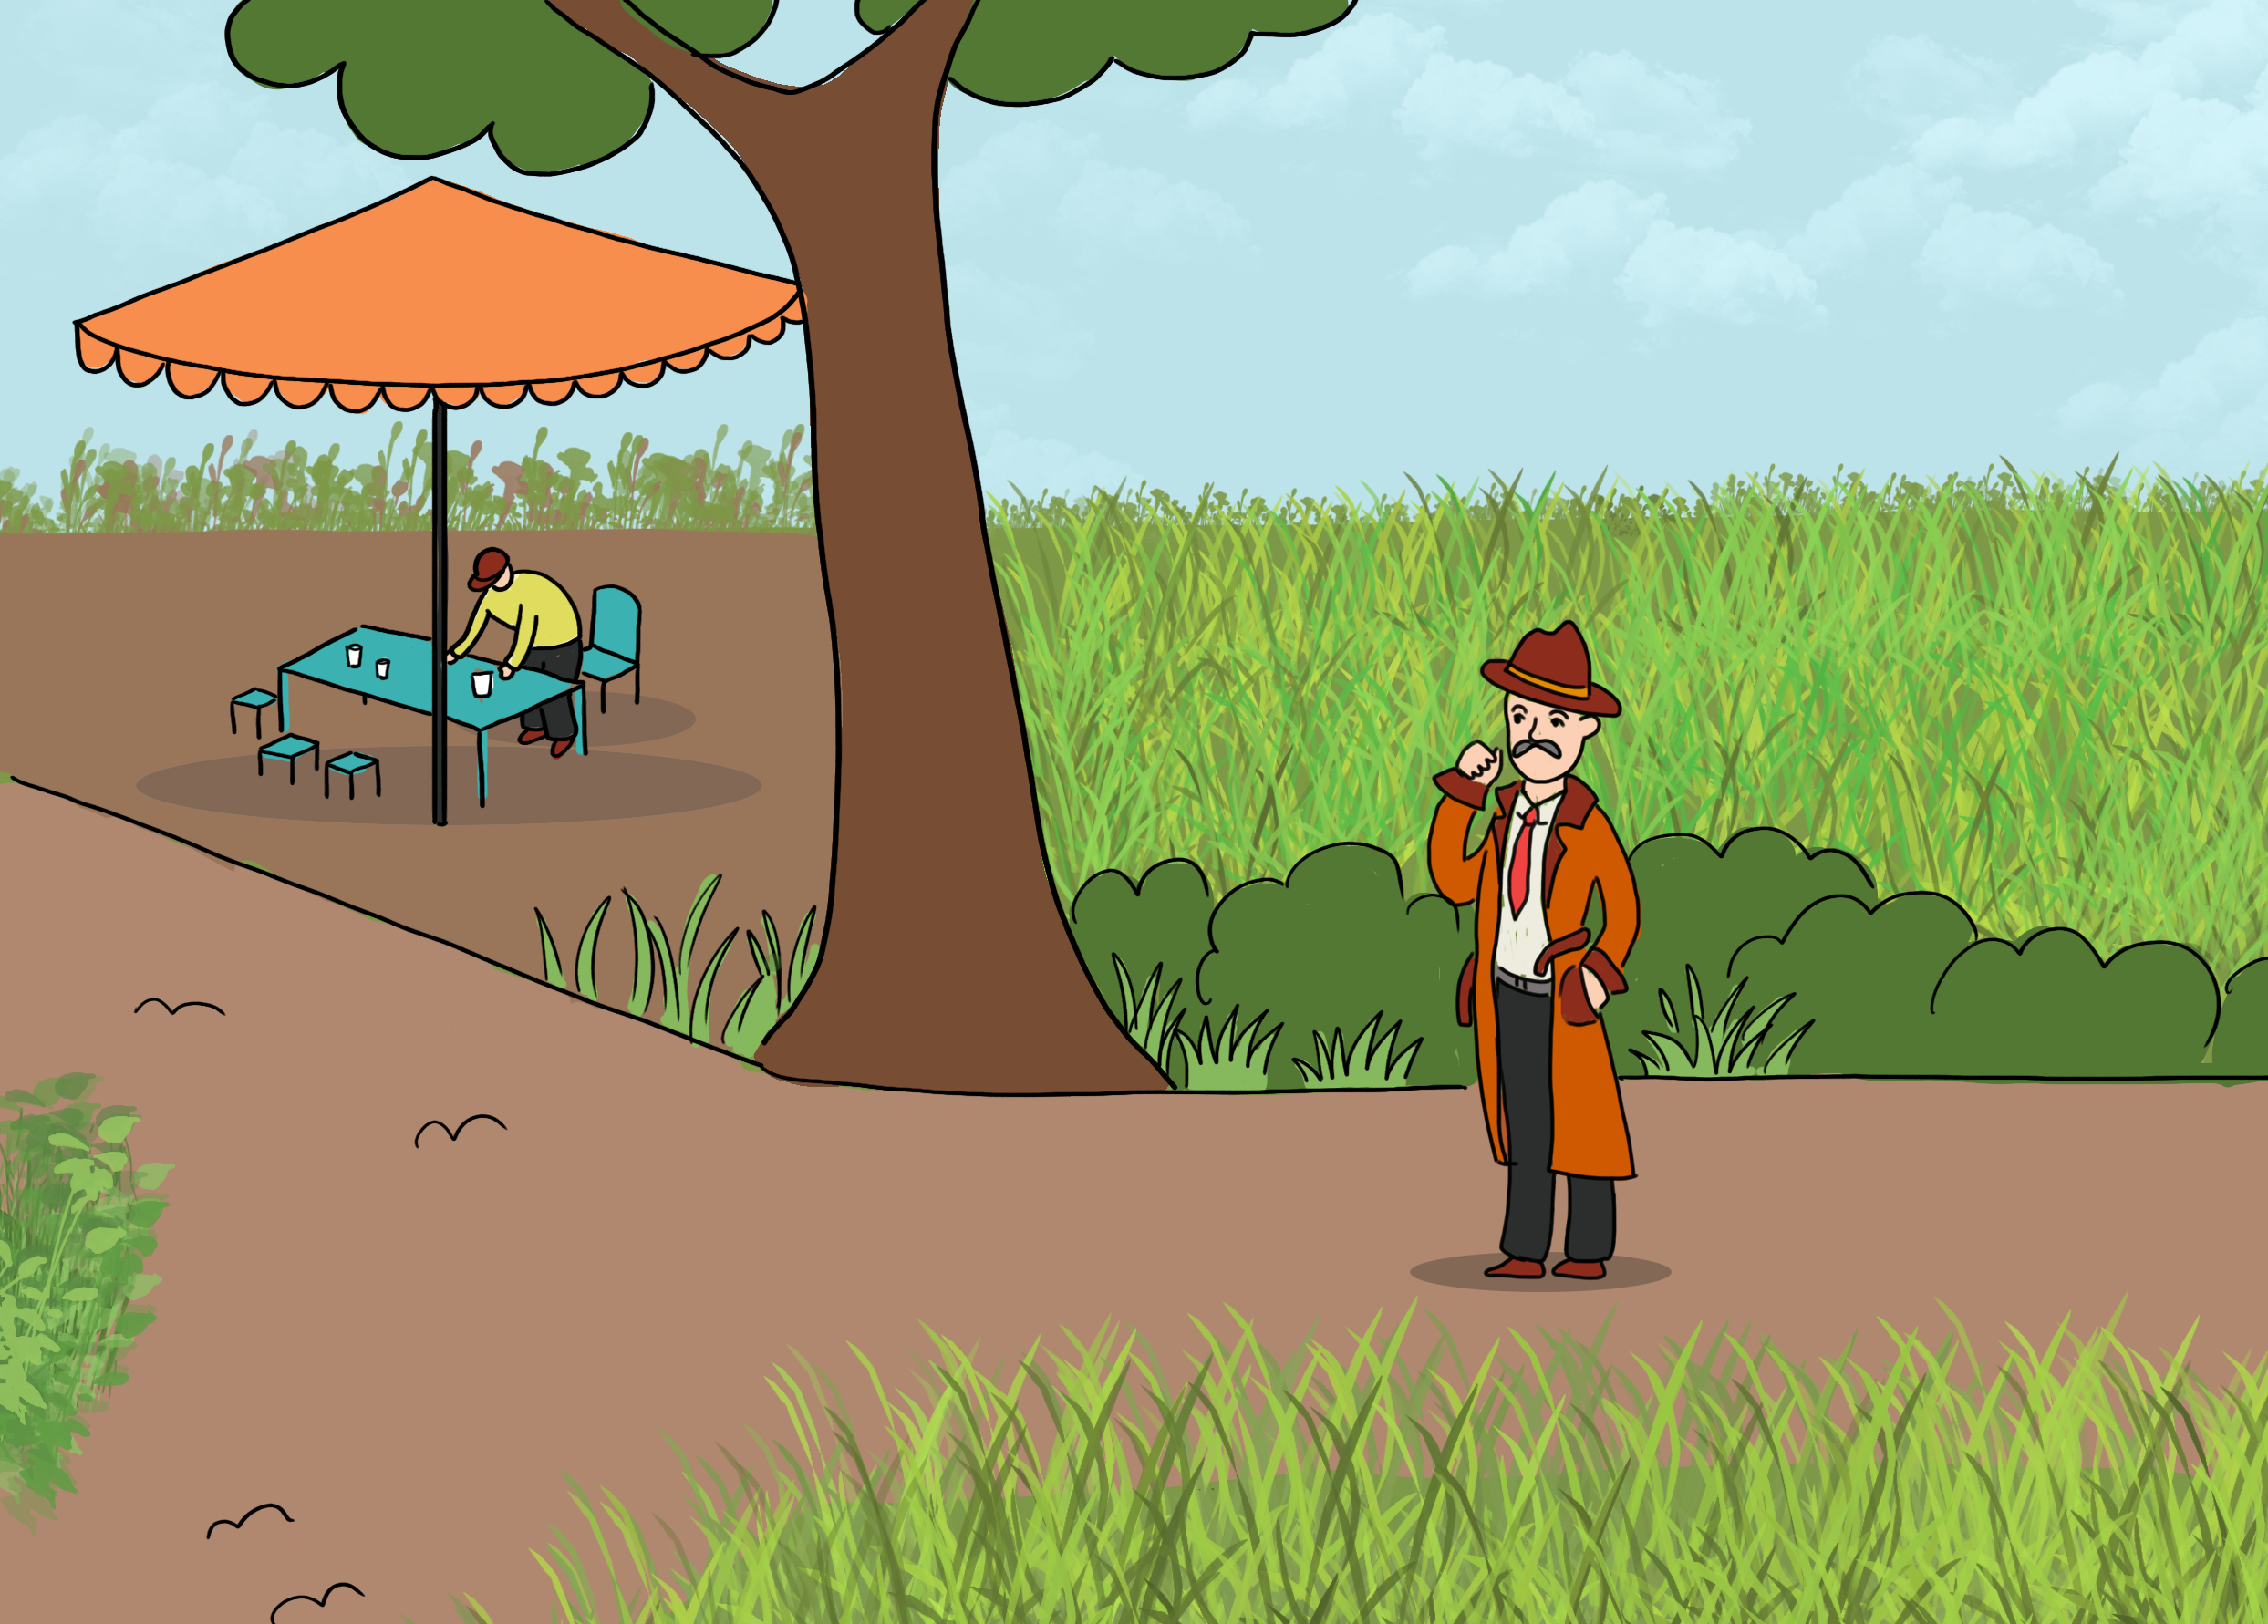
\includegraphics[width= 1\linewidth]{xp}
		\vspace*{-5pt}
	\end{figure}
\end{multicols}
\vspace*{-15pt}
\rule{1\linewidth}{0.1pt}
\begingroup
\AddToShipoutPicture*{\put(112,335){
\includegraphics[scale=1]{../tieude11.pdf}}} 
\centering
\endgroup
\vspace*{45pt}

\begin{multicols}{2}
	$\pmb{1.}$ Hai anh bạn rủ nhau đi câu cá. Khi được hỏi ``Trong mỗi giỏ của các anh có bao nhiêu con cá đấy?" thì anh thứ nhất trả lời ``Trong giỏ của tôi có số cá bằng nửa số cá ở giỏ của anh kia và thêm $10$ con nữa". Anh thứ hai lại nói ``Còn trong giỏ của tôi có số cá bằng số cá trong giỏ của anh kia và thêm $20$ con nữa". Vậy cả hai anh bạn có tất cả bao nhiêu con cá nhỉ? 
	\begin{figure}[H]
			\centering
			\vspace*{-10pt}
			\captionsetup{labelformat= empty, justification=centering}
			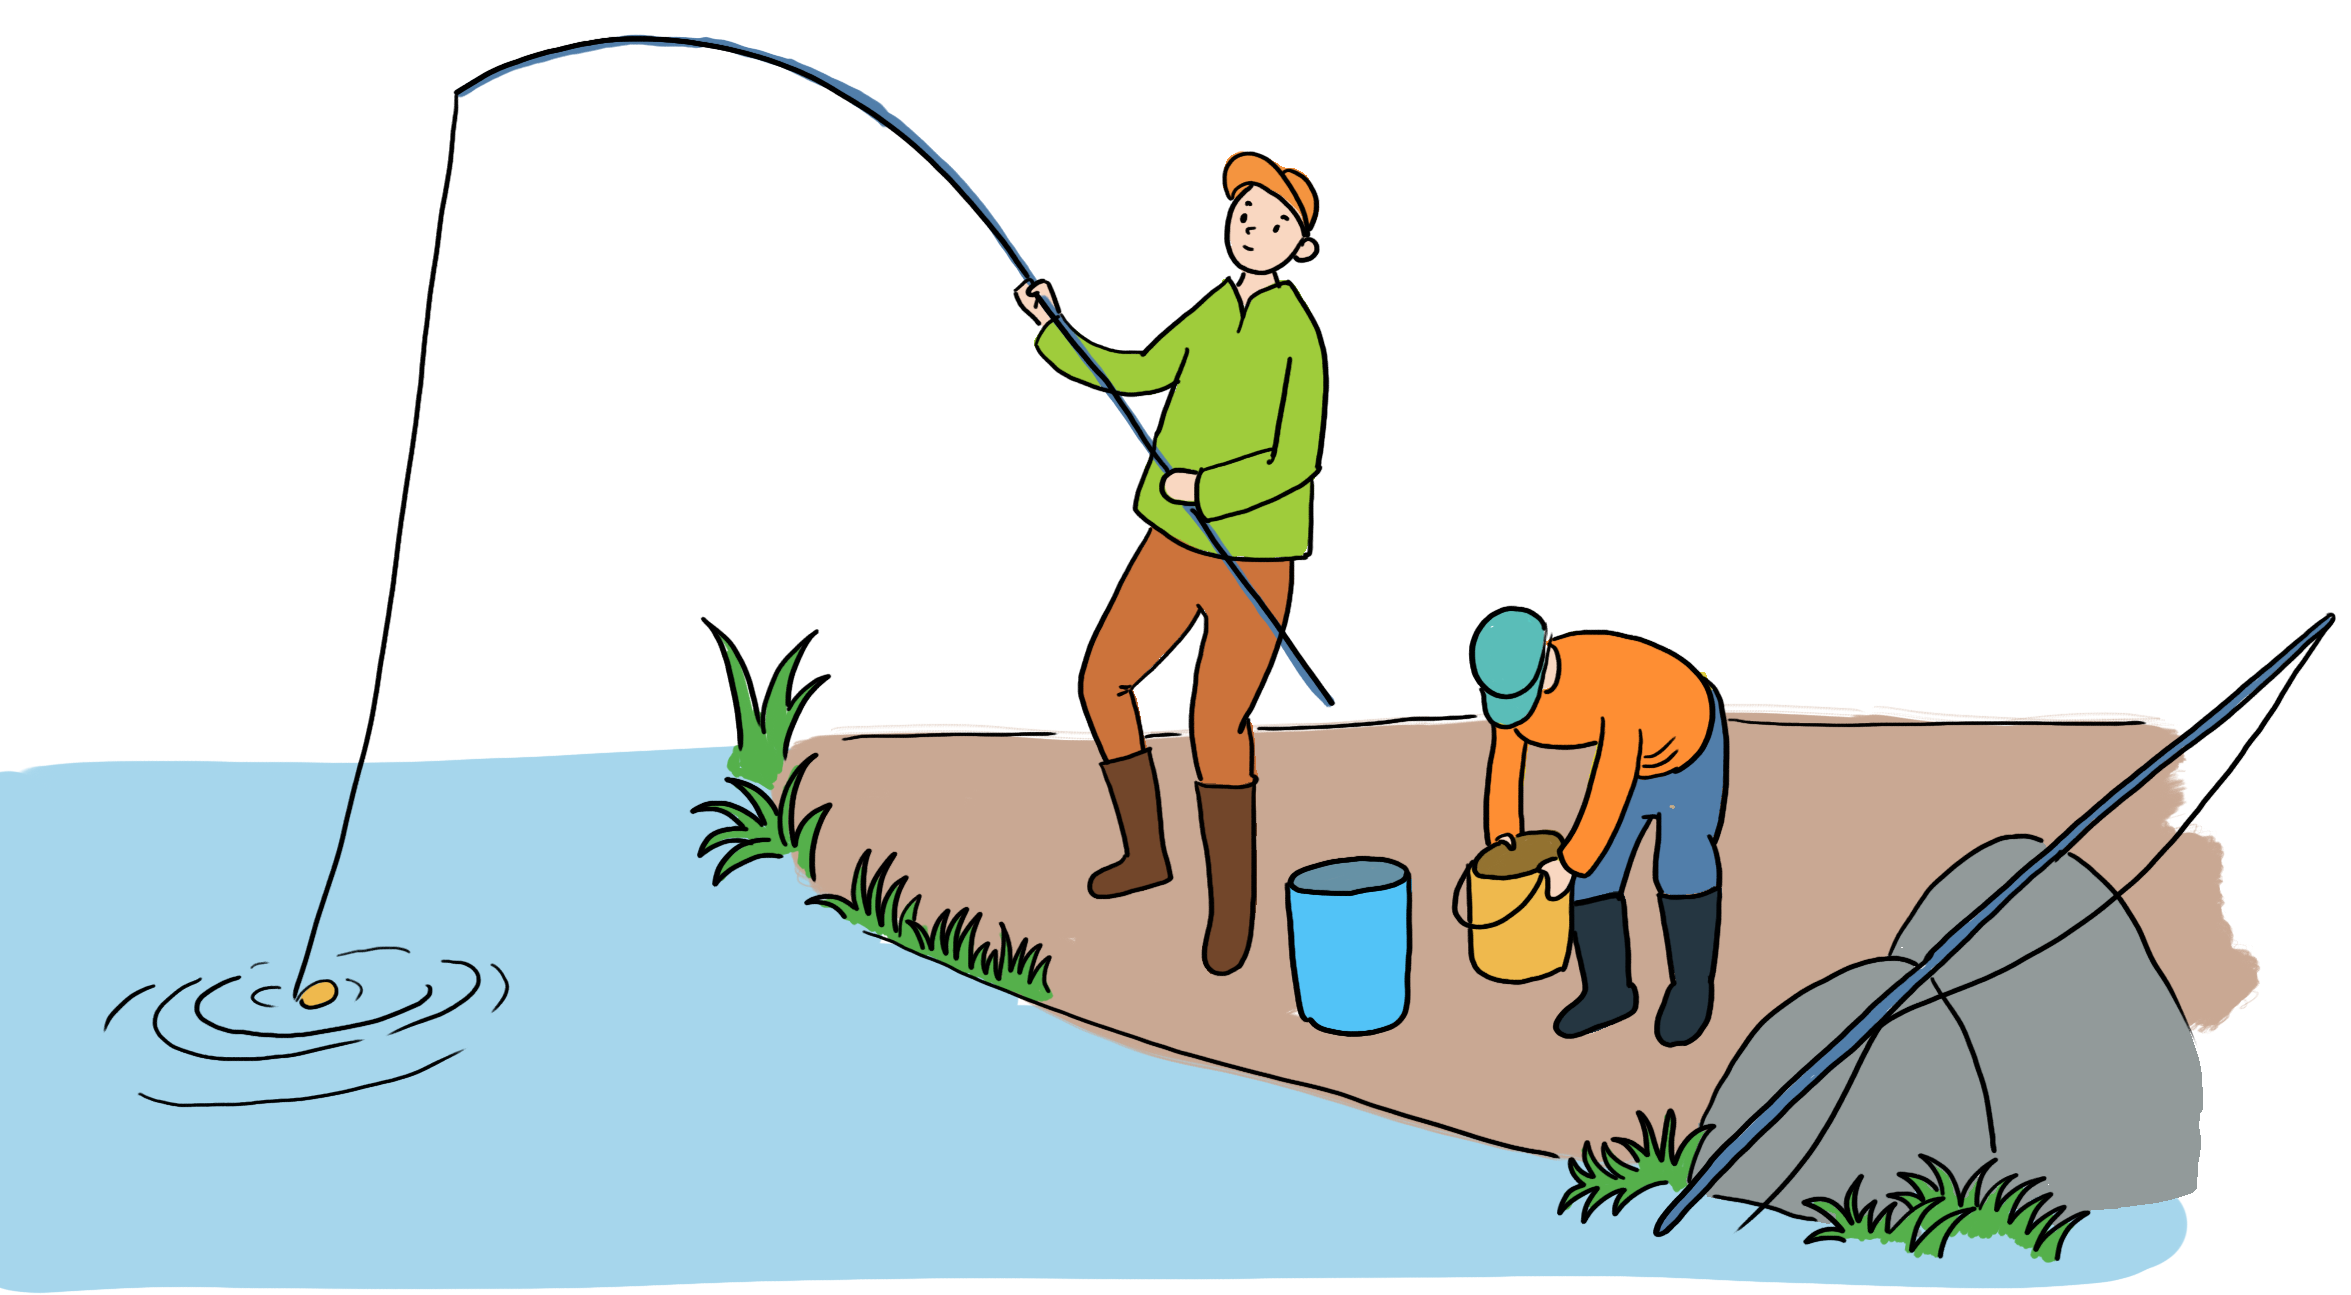
\includegraphics[width=1\linewidth]{Pi10_ToanBi_Bai1}
			\vspace*{-15pt}
		\end{figure}
	\vskip 0.1cm
	$\pmb{2.}$ Lọ lem có $100$  đựng hạt dẻ, lúc đầu số hạt dẻ trong mỗi rổ là như nhau. Lọ Lem lấy đi trong rổ thứ nhất một số hạt dẻ, lấy từ rổ  thứ hai một số gấp đôi như thế, lấy từ rổ thứ ba một số hạt gấp ba như thế, và cứ như vậy. Cuối cùng thì trong rổ thứ $100$ chỉ còn đúng một hạt dẻ, và còn lại ở tất cả trong 100 rổ tổng cộng là $14950$ hạt dẻ. Hỏi ban đầu trong mỗi rổ có bao nhiêu hạt dẻ?
	\begin{figure}[H]
			\centering
			\vspace*{-10pt}
			\captionsetup{labelformat= empty, justification=centering}
			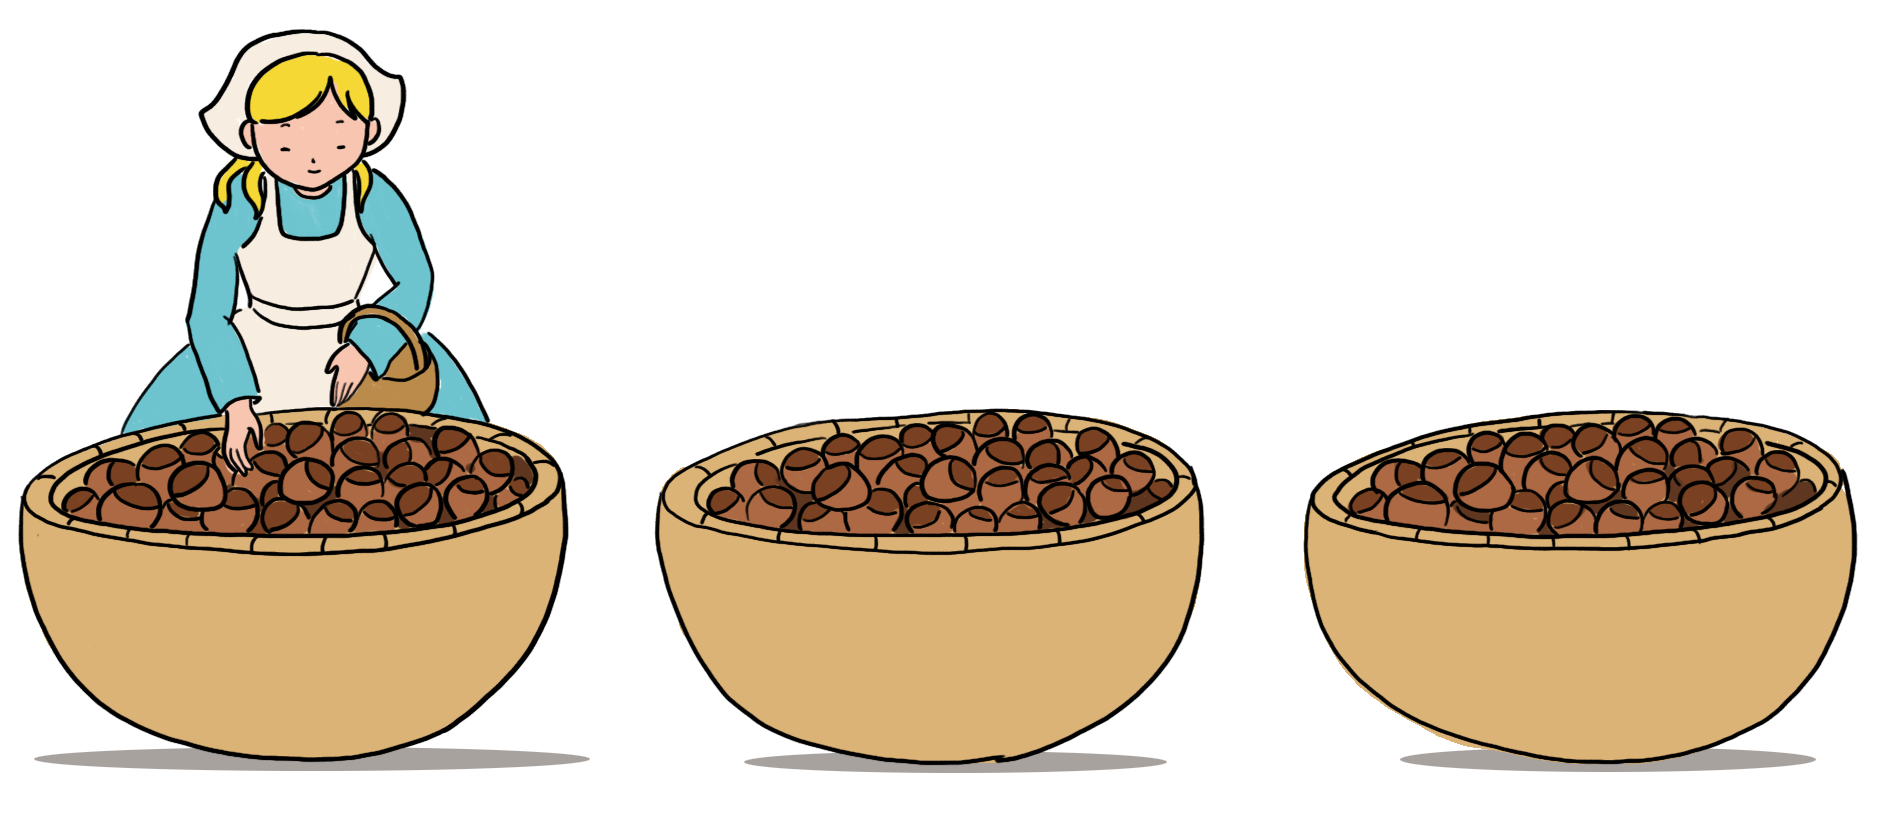
\includegraphics[width=0.97\linewidth]{Pi10_ToanBi_Bai2}
			\vspace*{-15pt}
		\end{figure}
	$\pmb{3.}$ Hai bạn học sinh là Nam và Vũ gặp nhau tại nhà của Vũ. Nam nói ``Nếu lấy số nhà của tớ là một số có hai chữ số trừ đi số có hai chữ số tạo thành khi viết theo thứ tự ngược lại, thì sẽ ra số nhà của cậu. Vậy tớ sống ở số nhà nào?"
	\vskip 0.1cm
	Vũ trả lời ``Ôi, bài toán này dễ quá" -- và giải ra luôn đáp số.
	\vskip 0.1cm
	Vậy các bạn đó sống ở những số nhà nào nhỉ?
	\begin{figure}[H]
			\centering
			\vspace*{-5pt}
			\captionsetup{labelformat= empty, justification=centering}
			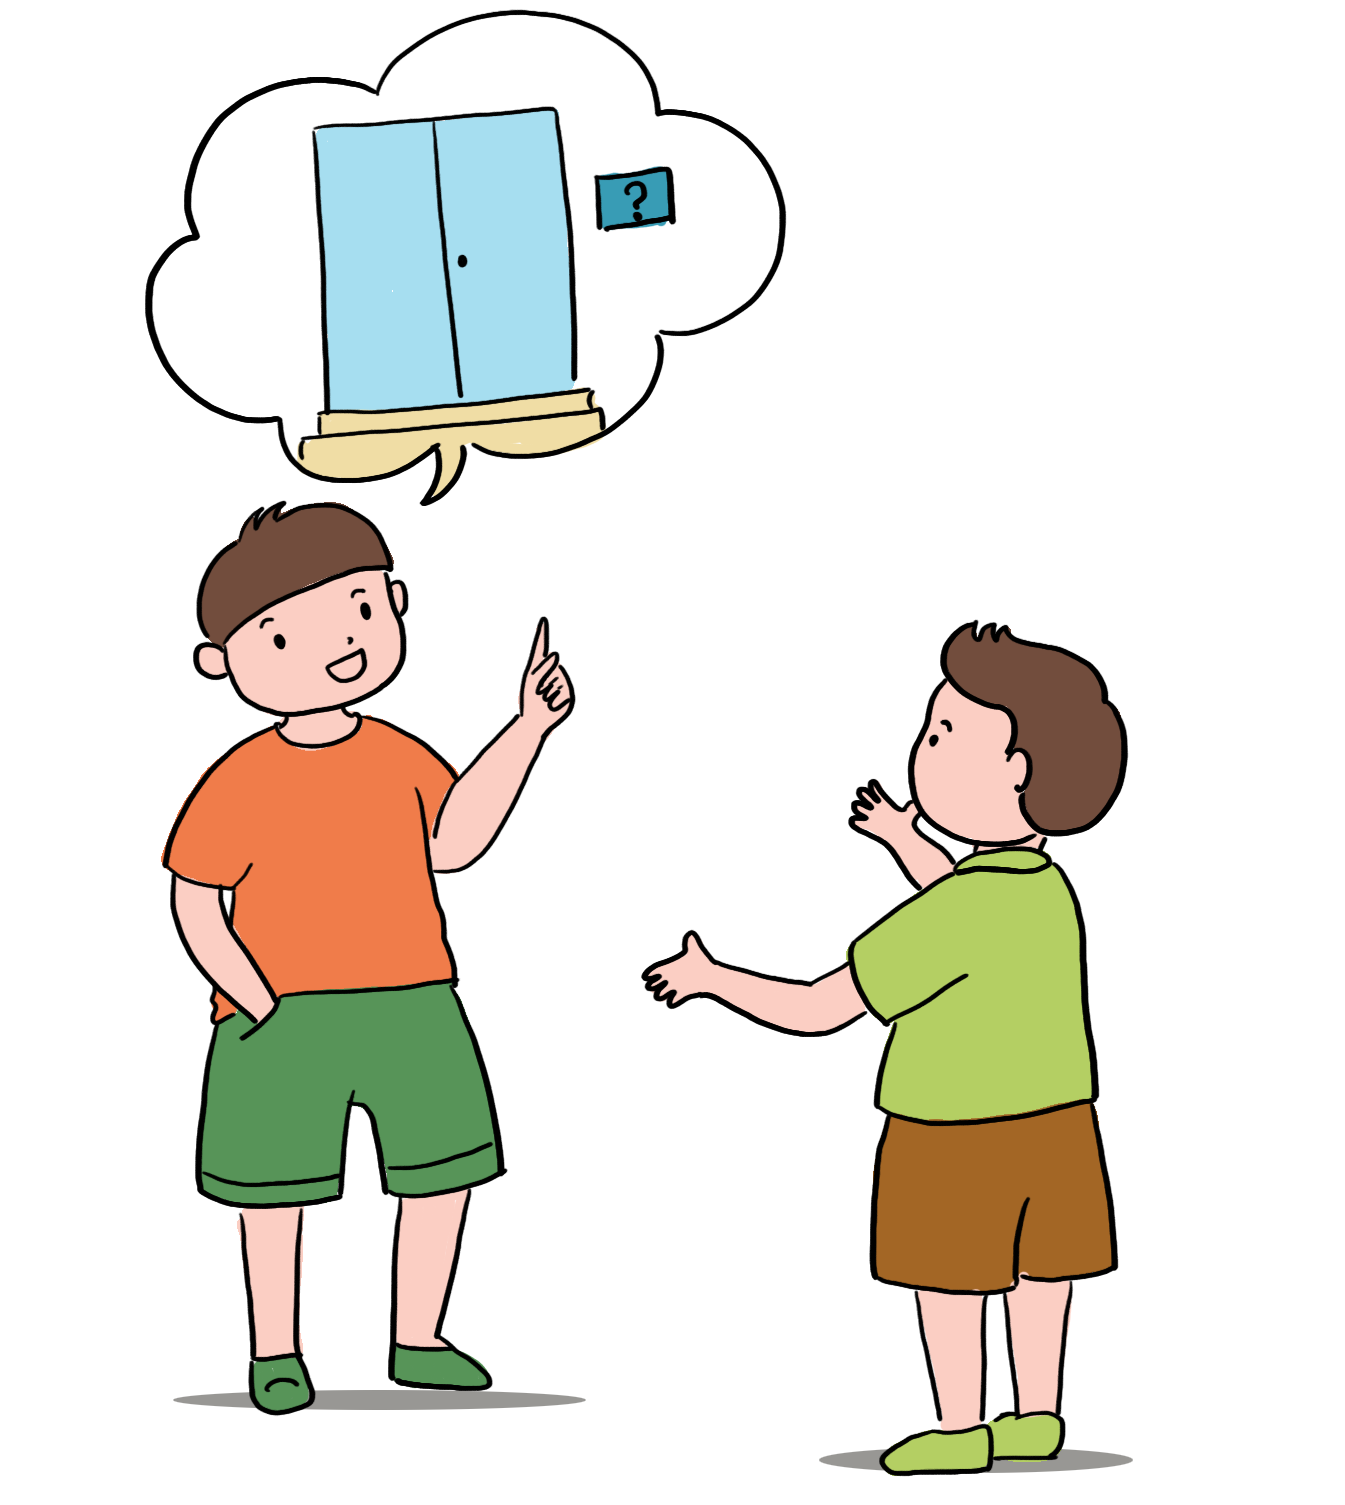
\includegraphics[width=0.7\linewidth]{Pi10_ToanBi_Bai3}
			\vspace*{-15pt}
		\end{figure}
	$\pmb{4.}$ Lớp của Hùng có $35$ học sinh. Trong số đó có $20$ em tham gia câu lạc bộ Toán, 11 em tham gia câu lạc bộ Khéo tay, $10$ em không tham gia vào hai nhóm này. Hỏi có tất cả bao nhiêu em vừa tham gia CLB Toán lại vẫn không quên tham gia cả CLB Khéo tay nhỉ?
	\begin{figure}[H]
			\centering
			\vspace*{-5pt}
			\captionsetup{labelformat= empty, justification=centering}
			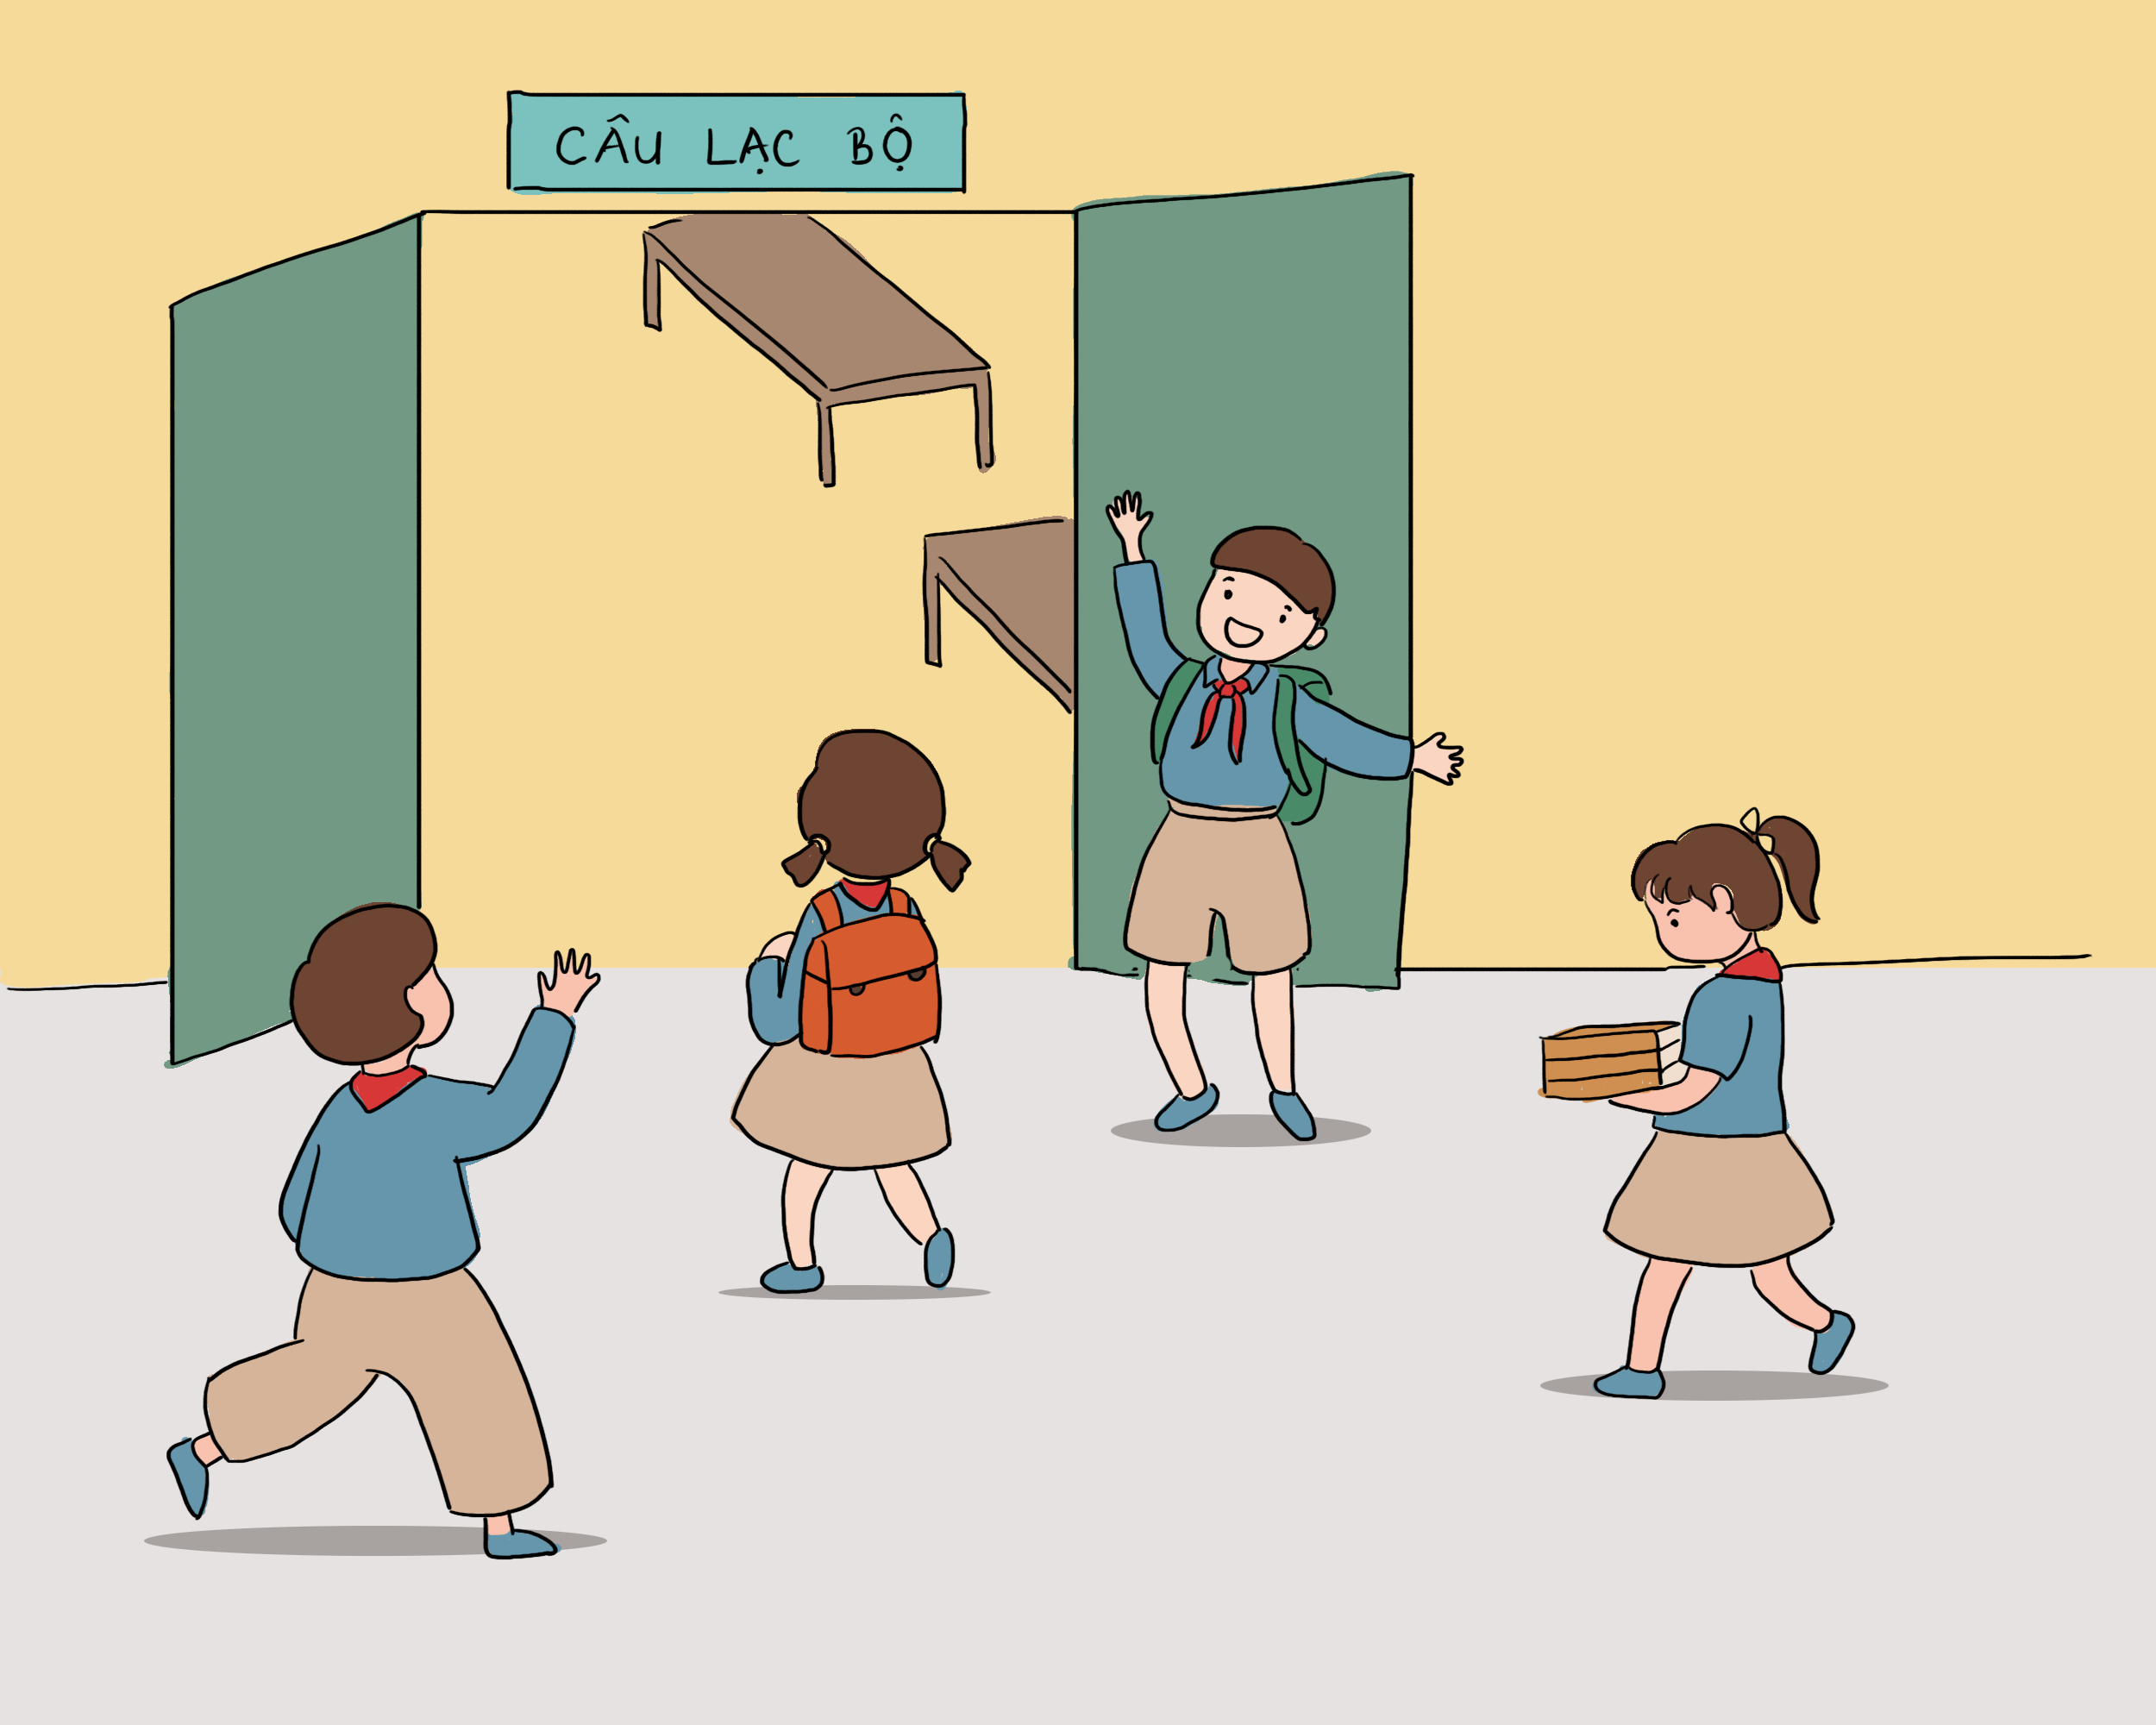
\includegraphics[width=1\linewidth]{Pi10_ToanBi_Bai4}
			\vspace*{-15pt}
		\end{figure}
	$\pmb{5.}$ Tùng đến trường mới có nhiều chuyện rất vui nên về khoe với bạn bè.
	\begin{figure}[H]
			\centering
	%		\vspace*{5pt}
			\captionsetup{labelformat= empty, justification=centering}
			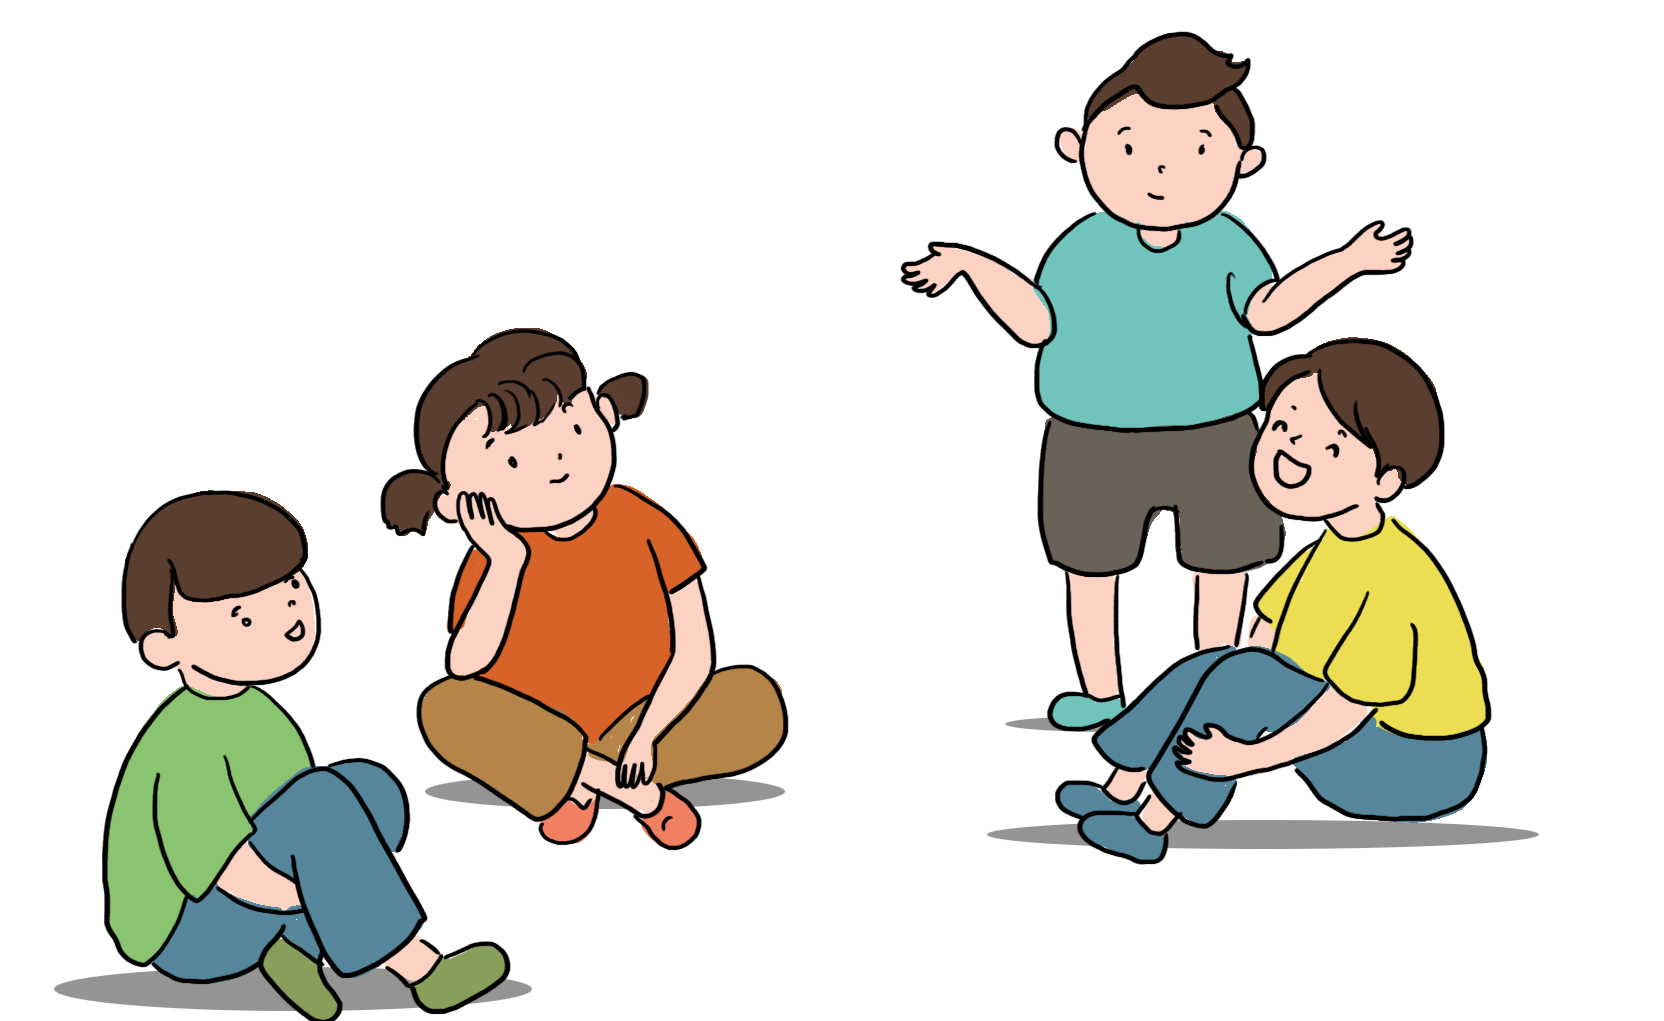
\includegraphics[width=1\linewidth]{Pi10_ToanBi_Bai5}
			\vspace*{-15pt}
		\end{figure}
	-- Lớp tớ có $35$ học sinh. Và cậu có tưởng tượng được không, mỗi người lại kết bạn với đúng $11$ học sinh cùng lớp.
	\vskip 0.1cm
	-- Không thể thế được! Bách, người bạn thân của Tùng vừa đạt giải trong một cuộc thi Olympic, ngay lập tức trả lời.
	\vskip 0.1cm
	Vì sao Bách lại nghĩ như vậy nhỉ?
	\vskip 0.1cm
	$\pmb{6.}$ Có $55$ em học sinh tham gia một cuộc thi Olympic. Tất cả các em đều nộp bài. Khi chấm bài, mỗi câu hỏi được chấm bởi một trong ba loại điểm: điểm ``$+$" nếu câu hỏi được trả lời hoàn toàn đúng; điểm ``$-$" nếu câu hỏi đã có trả lời nhưng chưa ra đúng đáp số; và điểm ``$0$" nếu câu hỏi chưa được trả lời. Sau khi chấm toàn bộ bài thi, ban tổ chức thấy không có hai bài thi nào có cả các số điểm ``$+$" và số điểm ``$-$" đồng thời trùng nhau. Vậy trong kỳ thi Olympic đó phải có ít nhất bao nhiêu câu hỏi?
\end{multicols}

\newpage
\begingroup
\AddToShipoutPicture*{\put(112,642){
\includegraphics[scale=1]{../tieude2.pdf}}} 
\centering
\endgroup
\graphicspath{{../toancuabi/pic/}}
\vspace*{60pt}

\begin{multicols}{2}
	$\pmb{1.}$ Một lần nọ, sau cơn mưa, bác Tuấn đi vào rừng để hái nấm. Bác khệ nệ bê được cả một sọt nấm nặng trĩu về. Nhưng thật buồn cho bác là về đến nhà, bác mới biết là trong số nấm tươi mới hái được thì có tới tận $90\%$ thành phần là nước, nên hoá ra bác mất công mang nước về suốt cả một quãng đường dài. Sau khi nấm được hong khô đi chút, khối lượng của đống nấm bị giảm đi $15$ kg, và bây giờ nước chỉ chiếm $60\%$ khối lượng. Hỏi lúc đầu bác Tuấn đã mang được bao nhiêu ki--lô--gam nấm từ rừng về nhà?
	\begin{figure}[H]
		\centering
		\vspace*{-10pt}
		\captionsetup{labelformat= empty, justification=centering}
		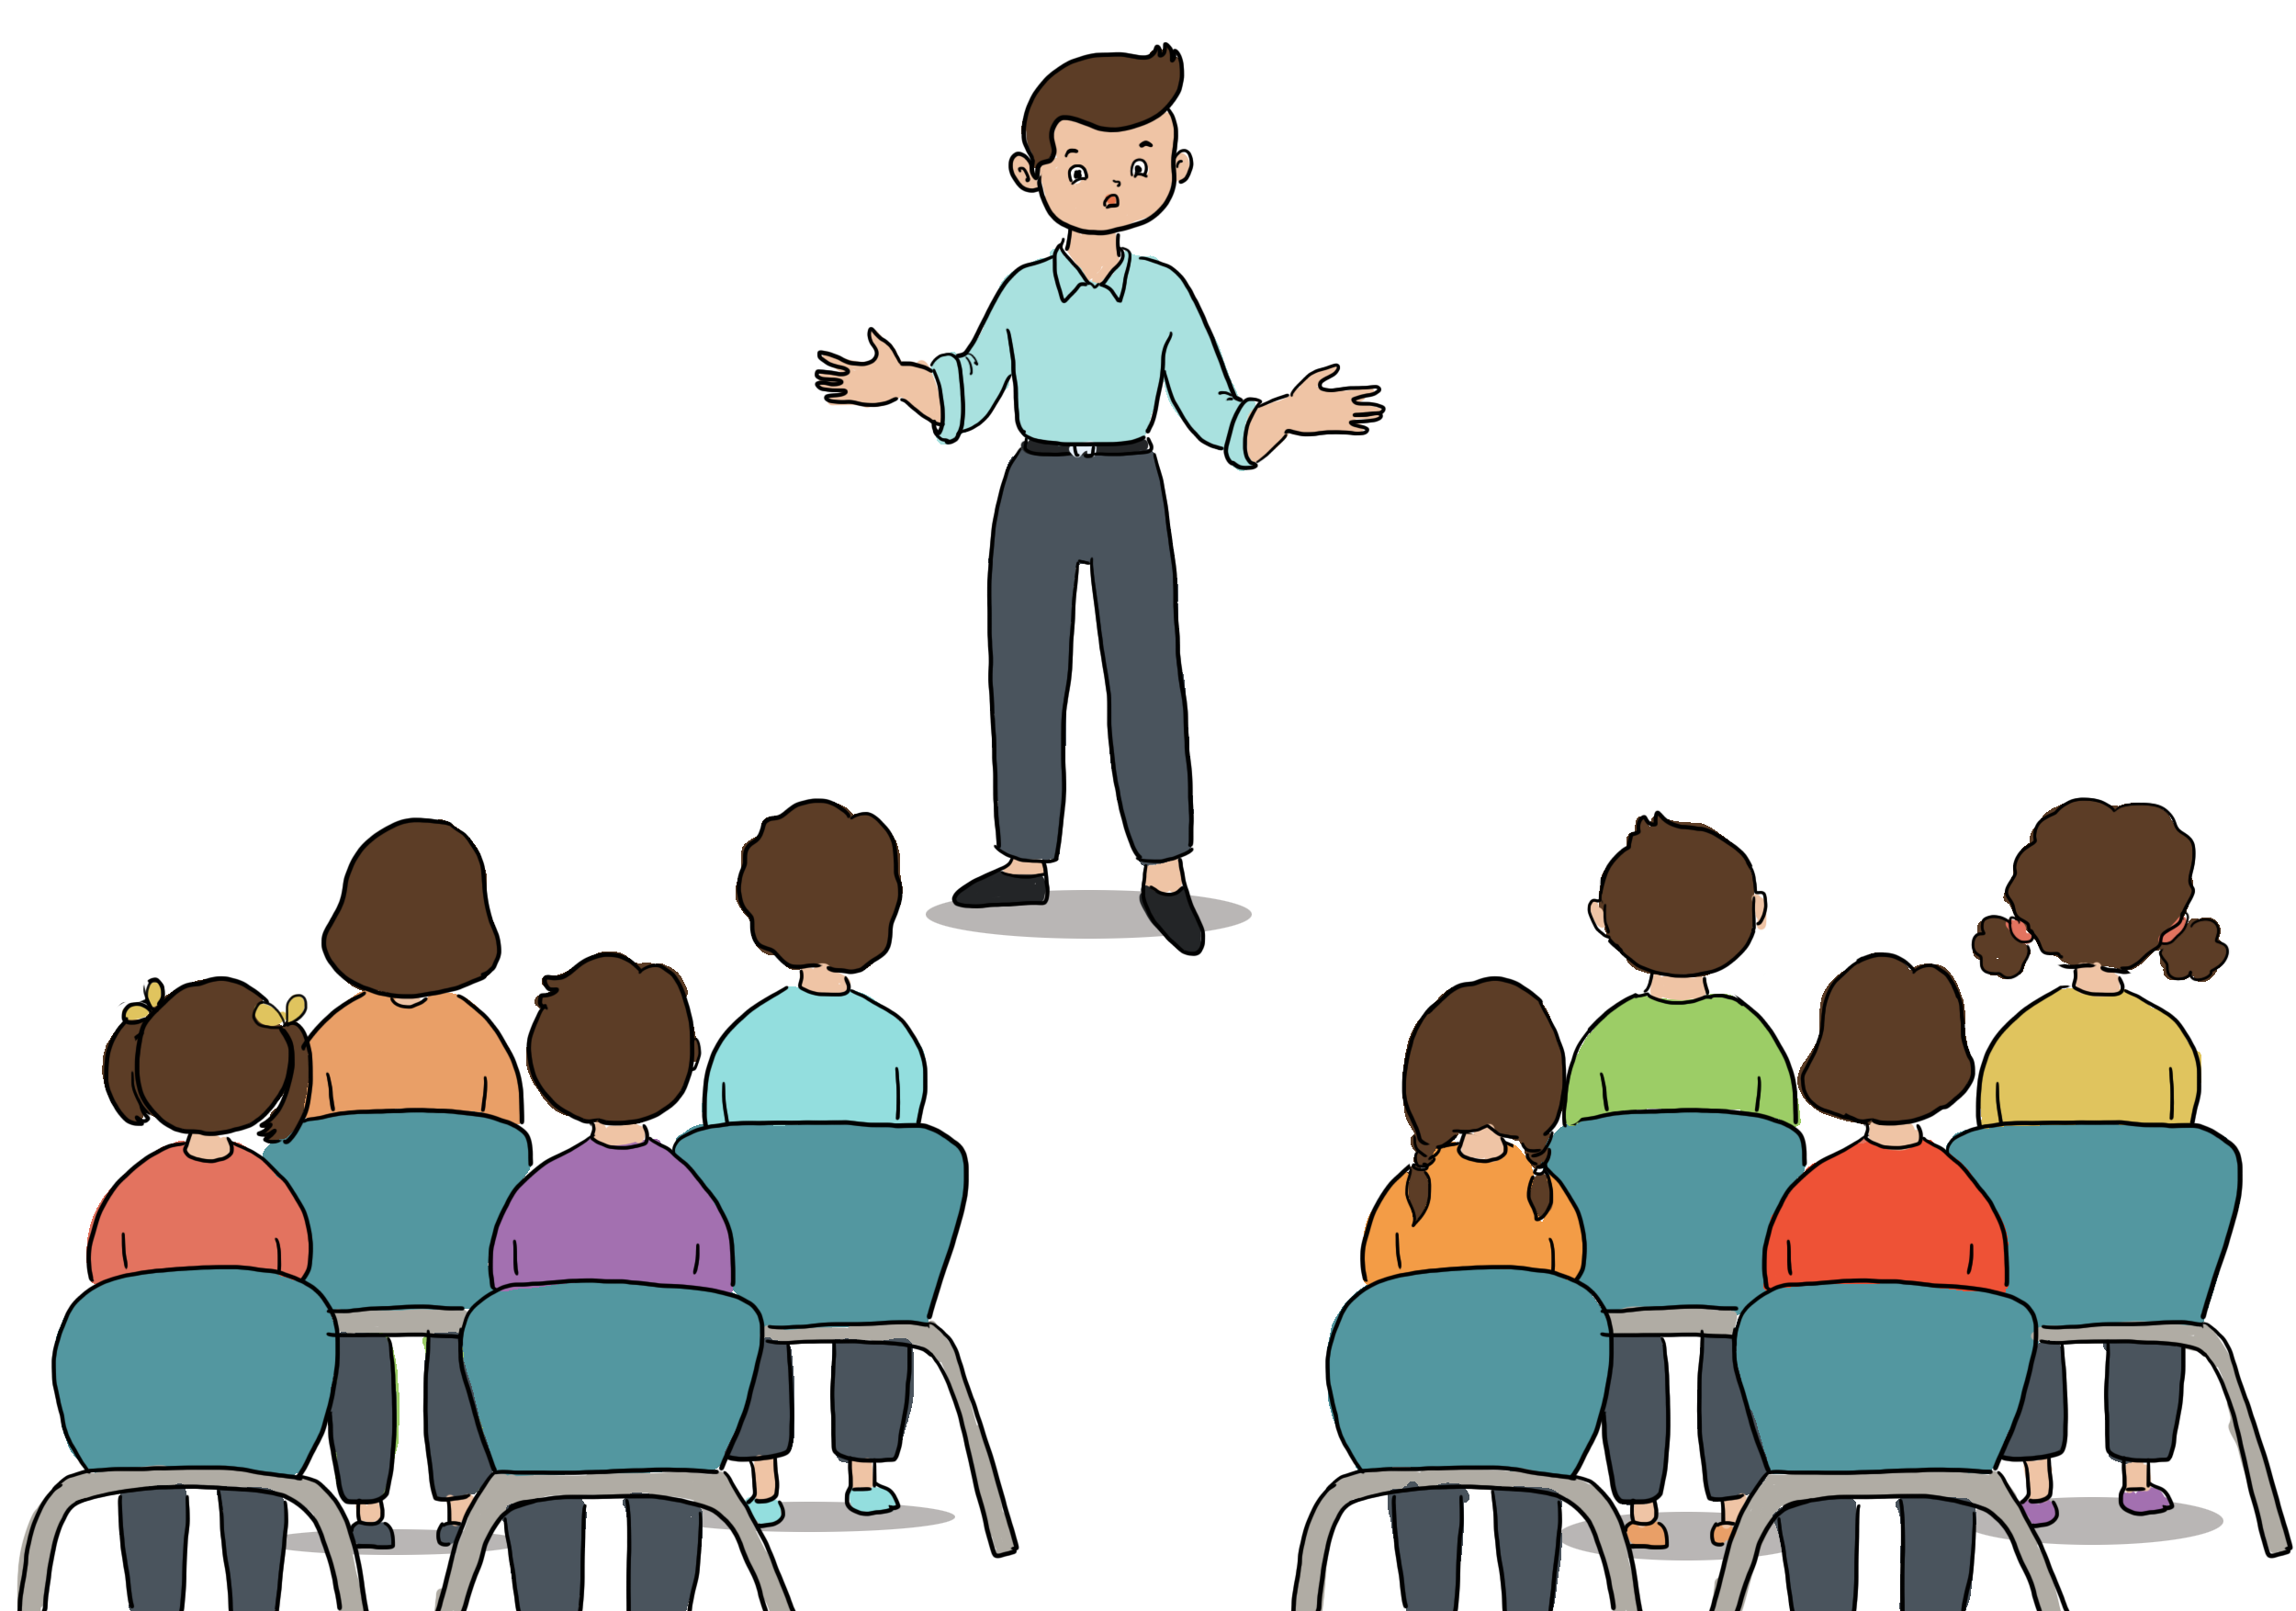
\includegraphics[width=0.4\linewidth]{bai1}
		\vspace*{-10pt}
	\end{figure}
	\textit{Lời giải.} 	Ta gọi $n$ là khối lượng nấm tinh khô nguyên chất. Khi đó lúc đầu trong đống nấm tươi mang về khối lượng nước là $9n$ và tổng khối lượng đống nấm tươi mà bác Tuấn đã mang về là $10n$ (kg). Sau khi hong khô, lượng nấm tinh khô chiếm $\frac{4}{10}$ lượng nấm tươi và do đó, khối lượng toàn đống nấm sau khi hong khô là $\frac{10n}{4}$, còn lượng nước còn lại sau khi hong khô là $\frac{6n}{4}$.
	\vskip 0.1cm
	Từ điều kiện suy ra $9n-\frac{6n}{4} =15$. Hay là $\frac{30n}{4}=15$. Từ đó ta có $n=2$. Suy ra lúc đầu khối lượng nấm mà bác Tuấn đã mang về là $20$ (kg).
	\vskip 0.1cm
	$\pmb{2.}$ Ông Ninh cùng với con trai mình và ông Phúc cùng với con trai mình đi ra hồ câu cá. Ông Ninh bắt được số con cá bằng với số con cá mà con trai ông  bắt được. Còn ông Phúc lại bắt được số con cá nhiều gấp ba lần số con cá mà con trai ông bắt được. Họ bắt được tổng cộng  $35$ con. Con trai của ông Ninh đi câu cá cùng ông tên là Giao. Hỏi con ông Phúc tên là gì và mỗi người hôm đó bắt được bao nhiêu con cá?
	\begin{figure}[H]
		\centering
		\vspace*{-15pt}
		\captionsetup{labelformat= empty, justification=centering}
		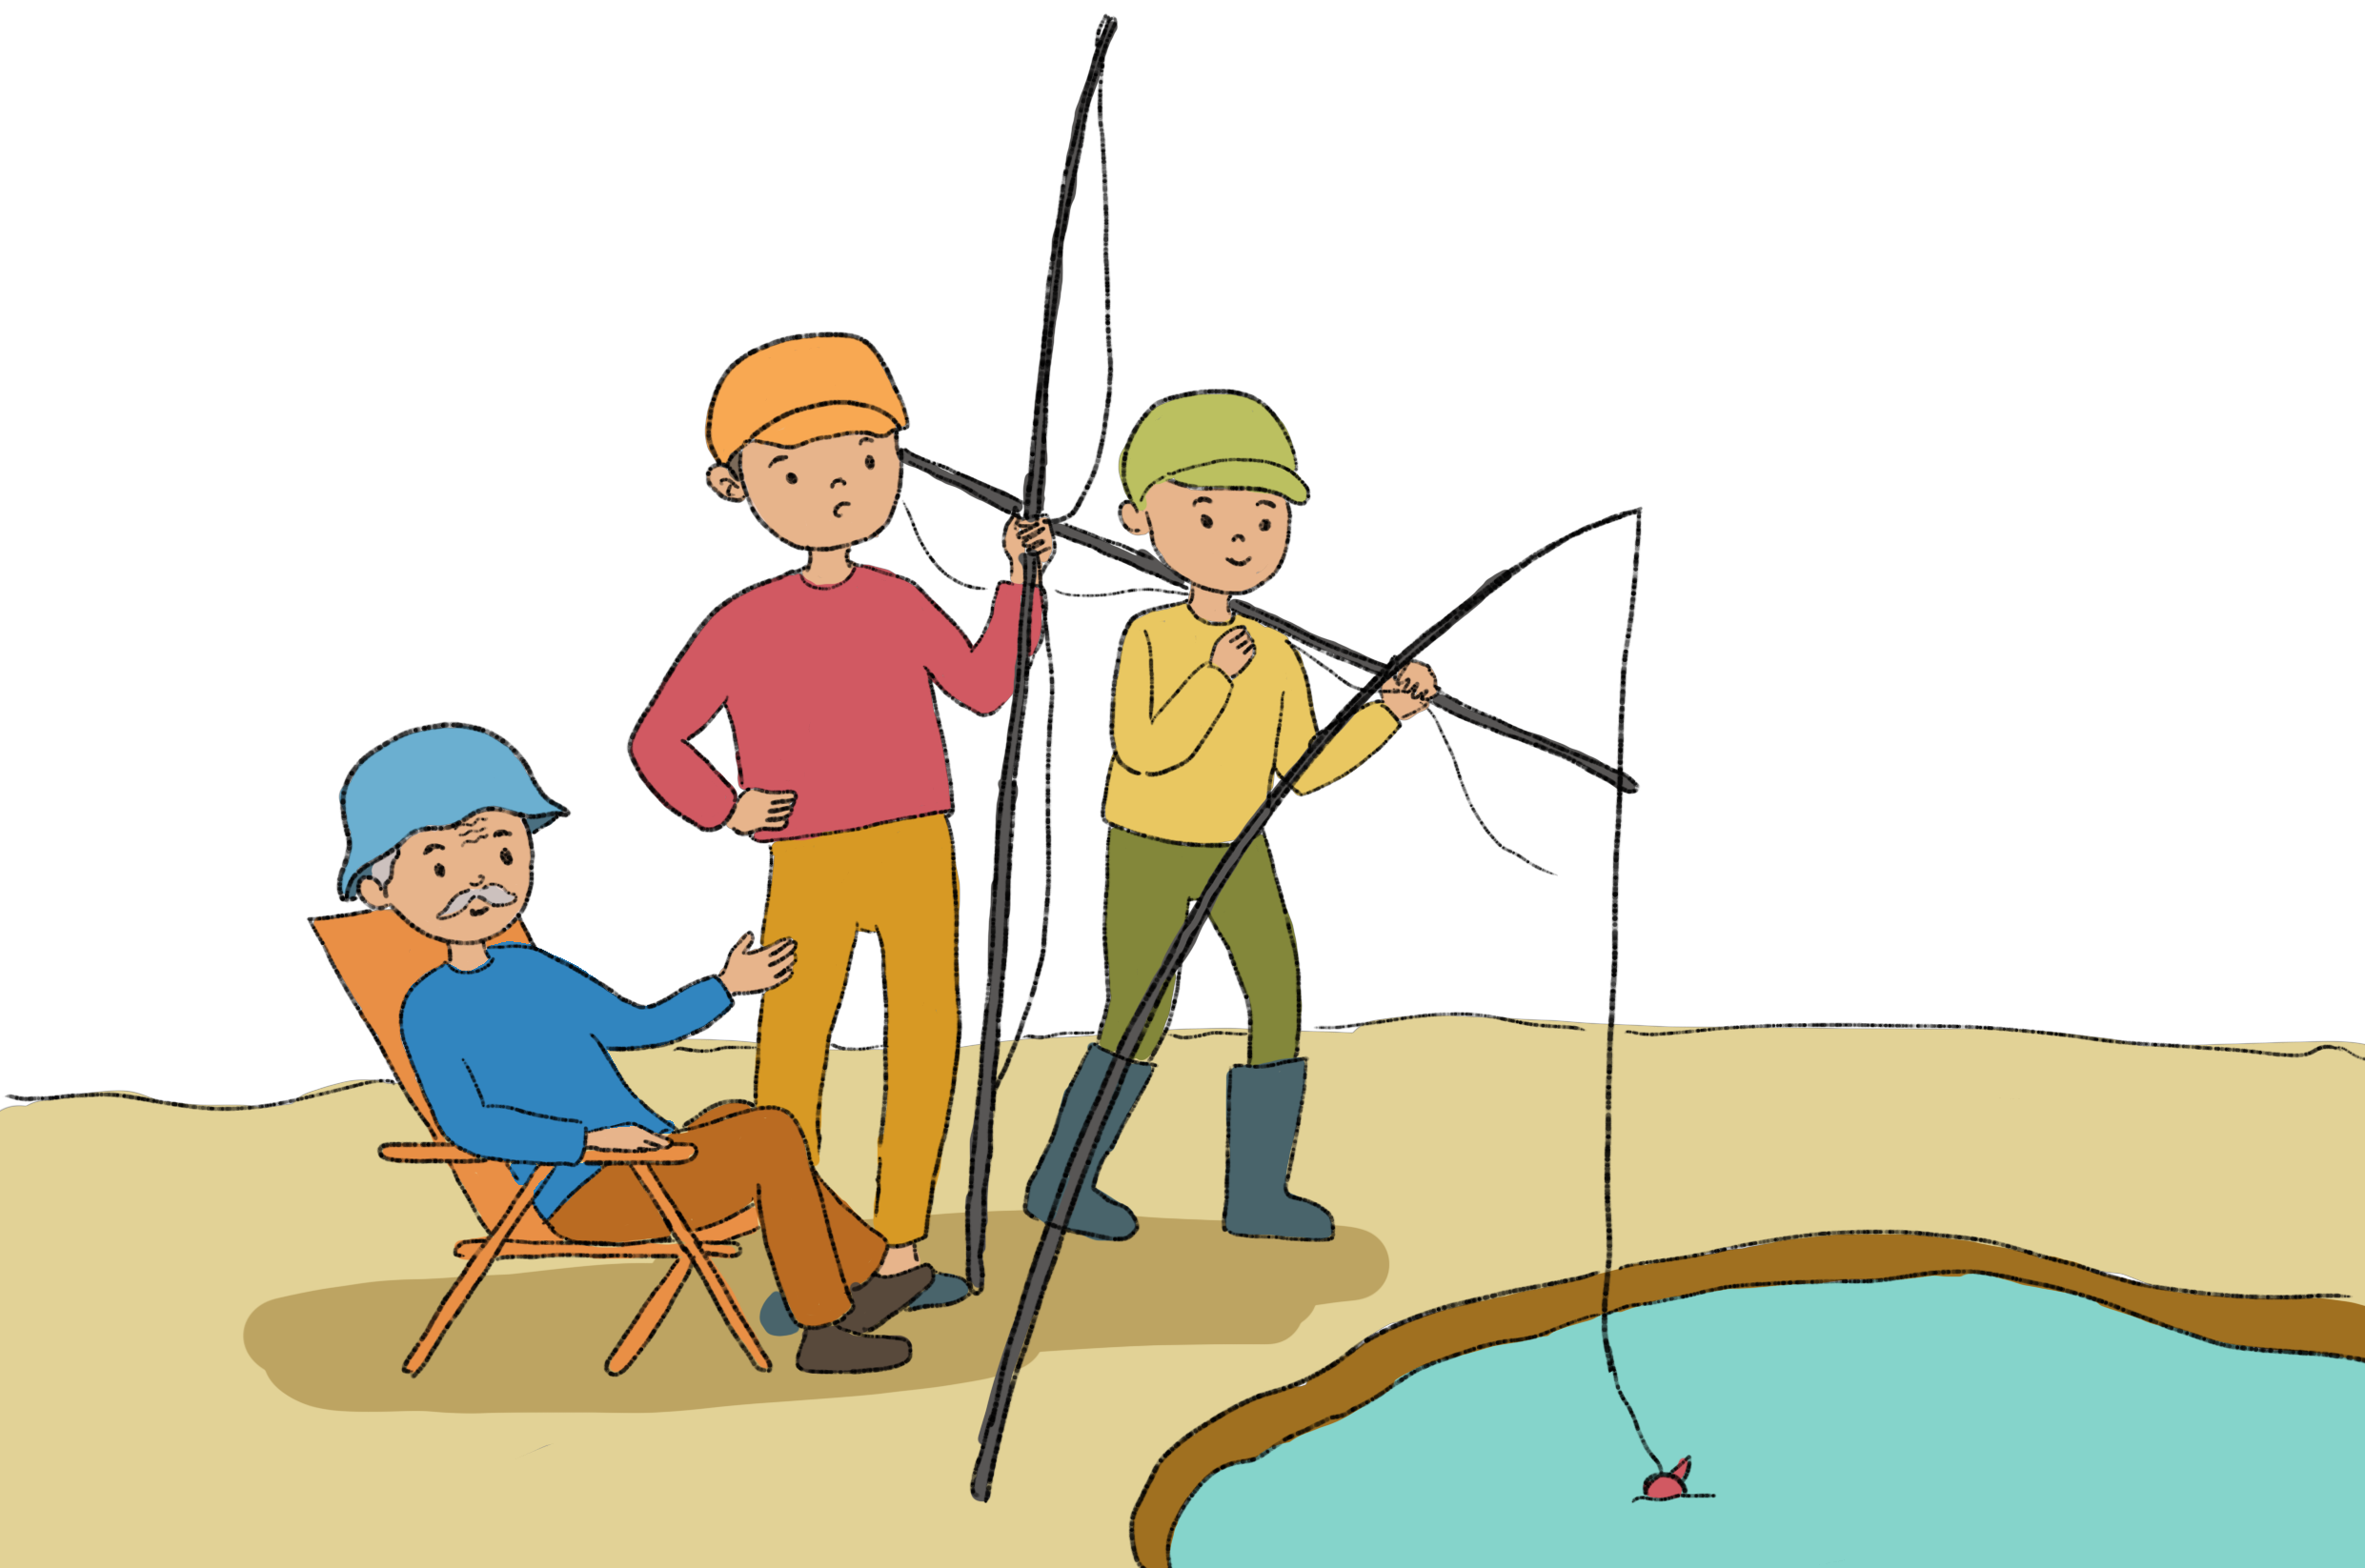
\includegraphics[width=1\linewidth]{bai2}
		\vspace*{-15pt}
		\end{figure}
	\textit{Lời giải.} 	Từ đề bài, nếu ký hiệu $a$ là số con cá mà con ông Ninh bắt được, còn $b$ là số con cá mà con ông Phúc bắt được thì ta có 
	\begin{align*}
			2a+4b = 35.
		\end{align*}
	Do đẳng thức trên không thể xảy ra với bất kỳ giá trị nguyên nào của $a$ và $b$, ta đi đến kết luận rằng chỉ có $3$ người ra hồ câu cá chứ không phải $4$ người. Tuy nhiên do con trai của ông Ninh tên là Giao, ta loại được trường hợp ông Phúc là con của ông Ninh. Vì vậy ba người đó là: ông Phúc, con trai ông ta là ông Ninh,  và cháu nội ông Phúc là Giao. Ta kết luận được con của ông Phúc tên là Ninh.
	\vskip 0.1cm
	Ta thấy tổng số cá $3$ người bắt là $a+a+3a=5a = 35$. Từ đó dễ thấy Giao và ông Ninh mỗi người bắt được $7$ con cá, còn ông Phúc bắt được $21$ con cá.
	\vskip 0.1cm
	$\pmb{3.}$ Chiếc đồng hồ treo tường nhà bạn Lâm chỉ  $9$ giờ $20$ phút. Hỏi lúc đó góc tạo bởi kim giờ và kim phút bằng bao nhiêu độ (góc tương ứng với một vòng tròn là $360$ độ)?
	
%	\begin{figure}[H]
%			\centering
%			\vspace*{-10pt}
%			\captionsetup{labelformat= empty, justification=centering}
%			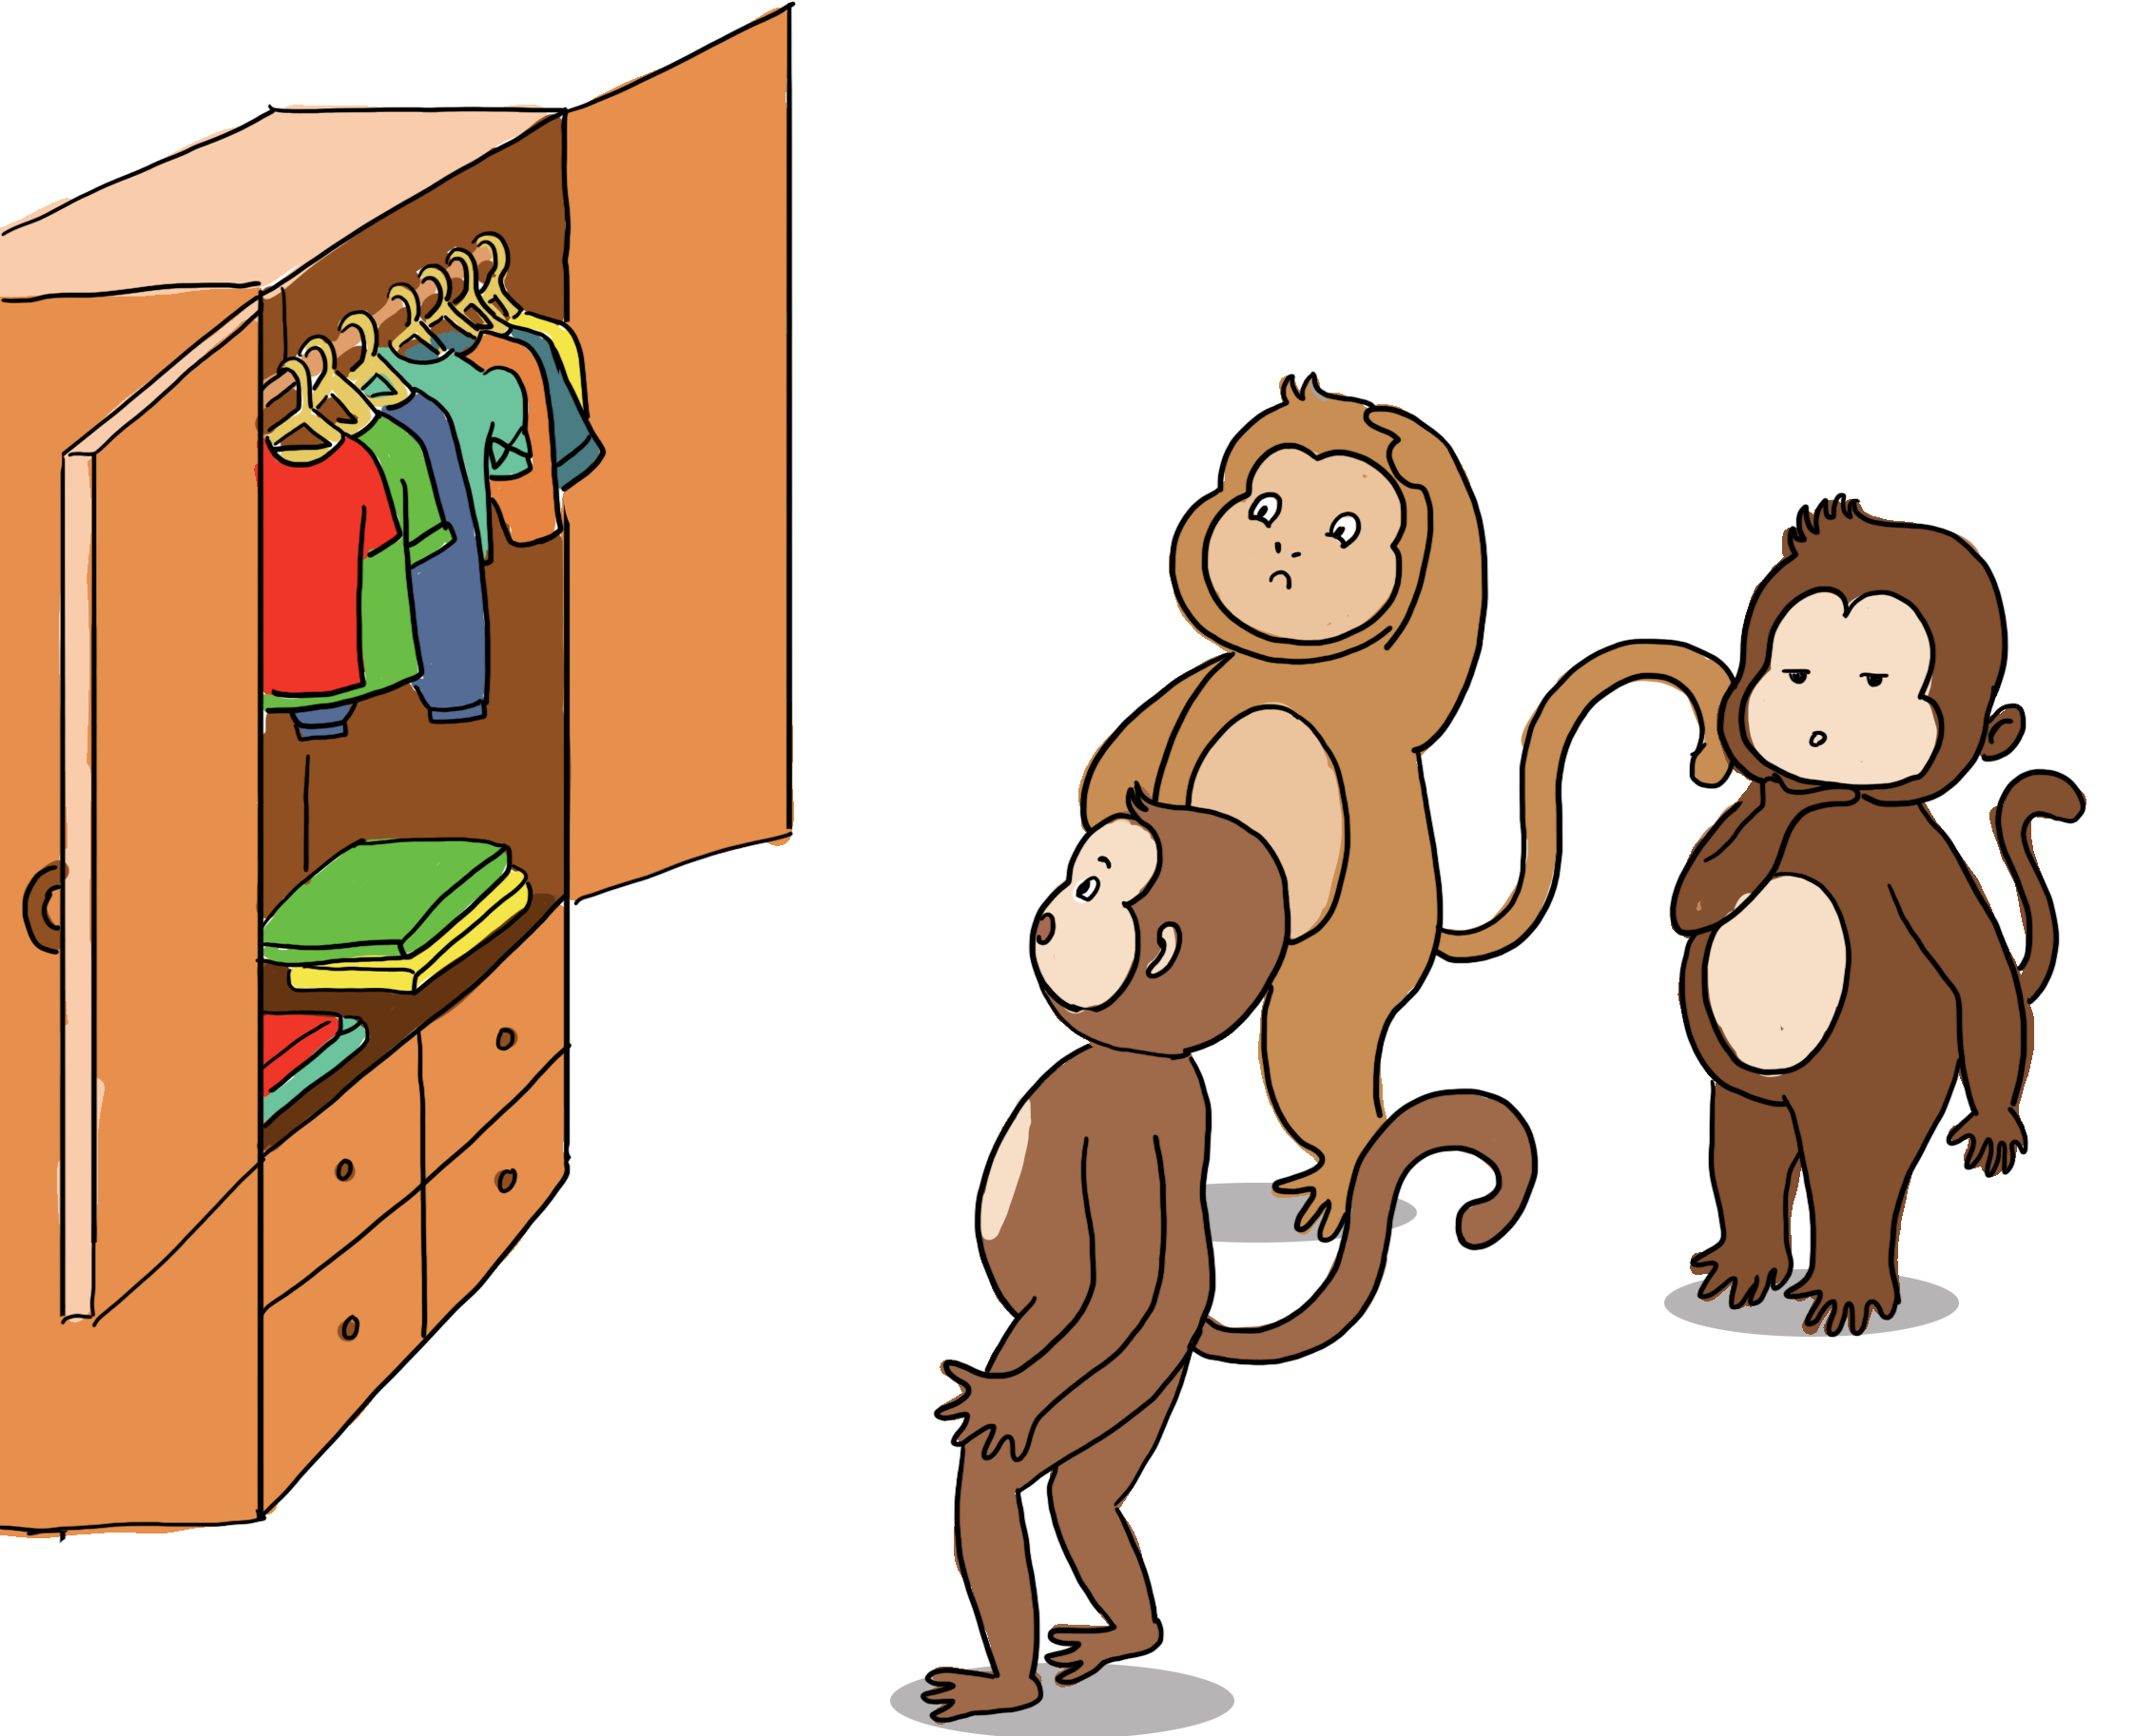
\includegraphics[width=0.8\linewidth]{bai3}
%			\vspace*{-15pt}
%		\end{figure}
	\textit{Lời giải.} 	Vào lúc $9$ giờ góc tạo bởi $2$ kim giờ và kim phút là $90^\circ$. Trong một tiếng, kim giờ đi được $\frac{1}{12}$ vòng tròn, có nghĩa là $\frac{1}{12}\times 360^\circ = 30^\circ$. Như vậy trong $20$ phút, kim giờ đi được $\frac{1}{3}$ quãng đường này, có nghĩa là $\frac{1}{3}\times 30^\circ=10^\circ$. Tương tự như vậy, sau một tiếng, kim phút đi được $360^\circ$ và do đó sau $20$ phút, nó quay được một góc bằng $\frac{20}{60}\times 360^\circ=120^\circ$. Vì thế, đến lúc $9$ giờ $20$ phút góc tạo bởi hai kim bị giảm đi $10^\circ$ nhưng lại tăng thêm $120^\circ$, điều này có nghĩa là nó sẽ bằng $90^\circ-10^\circ+120^\circ=200^\circ$. Nếu ta lấy góc bổ sung với nó theo quy ước với những góc lớn hơn góc bẹt, thì góc tạo bởi hai kim sẽ bằng $360^\circ-200^\circ=160^\circ$.
	\vskip 0.1cm
	$\pmb{4.}$ Tích của một tỷ số tự nhiên bằng đúng $1$ tỷ. Hỏi giá trị lớn nhất của tổng của chúng bằng bao nhiêu?
	\begin{figure}[H]
			\centering
			\vspace*{-10pt}
			\captionsetup{labelformat= empty, justification=centering}
			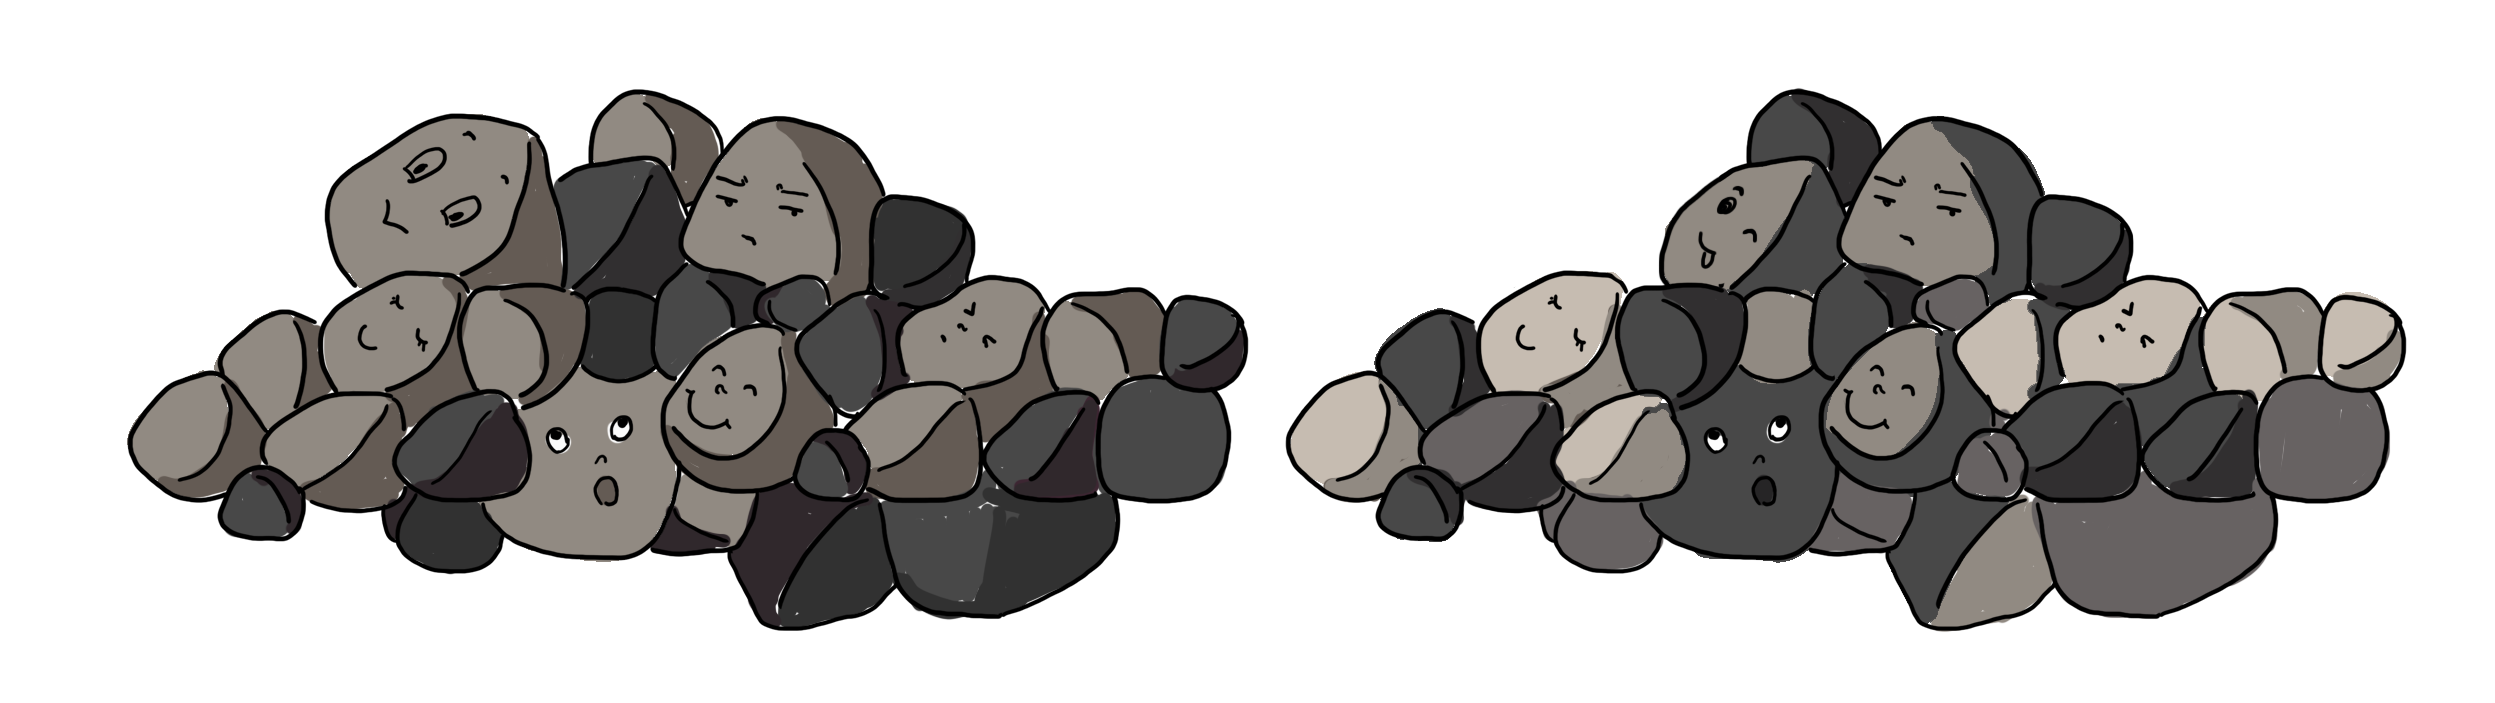
\includegraphics[width=0.7\linewidth]{bai5}
			\vspace*{-10pt}
		\end{figure}
	\textit{Lời giải.} 	Nếu trong số các số tự nhiên đã cho có hai số $a$ và $b$ cùng lớn hơn $1$, thì thay hai số $(a,b)$ bởi cặp $(ab,1)$ ta nhận được tích của các số không thay đổi, nhưng tổng  sẽ tăng, do từ $(a-1)(b-1) >0$ suy ra $ab+1 > a+b$. Vì thế tổng các số này sẽ lớn nhất nếu có một số bằng $1$ tỷ, còn tất cả các số còn lại đều bằng đơn vị. Do đó tổng của các số có giá trị lớn nhất bằng $1 999 999 999$.
	\vskip 0.1cm
	$\pmb{5.}$ Làm thế nào để xác định tâm của một hình tròn nếu chỉ có một cái bút chì và một cái thước kẻ thông thường có hai cạnh song song (chiều rộng của thước kẻ nhỏ hơn đường kính của hình tròn).
	\begin{figure}[H]
			\centering
			\vspace*{-10pt}
			\captionsetup{labelformat= empty, justification=centering}
			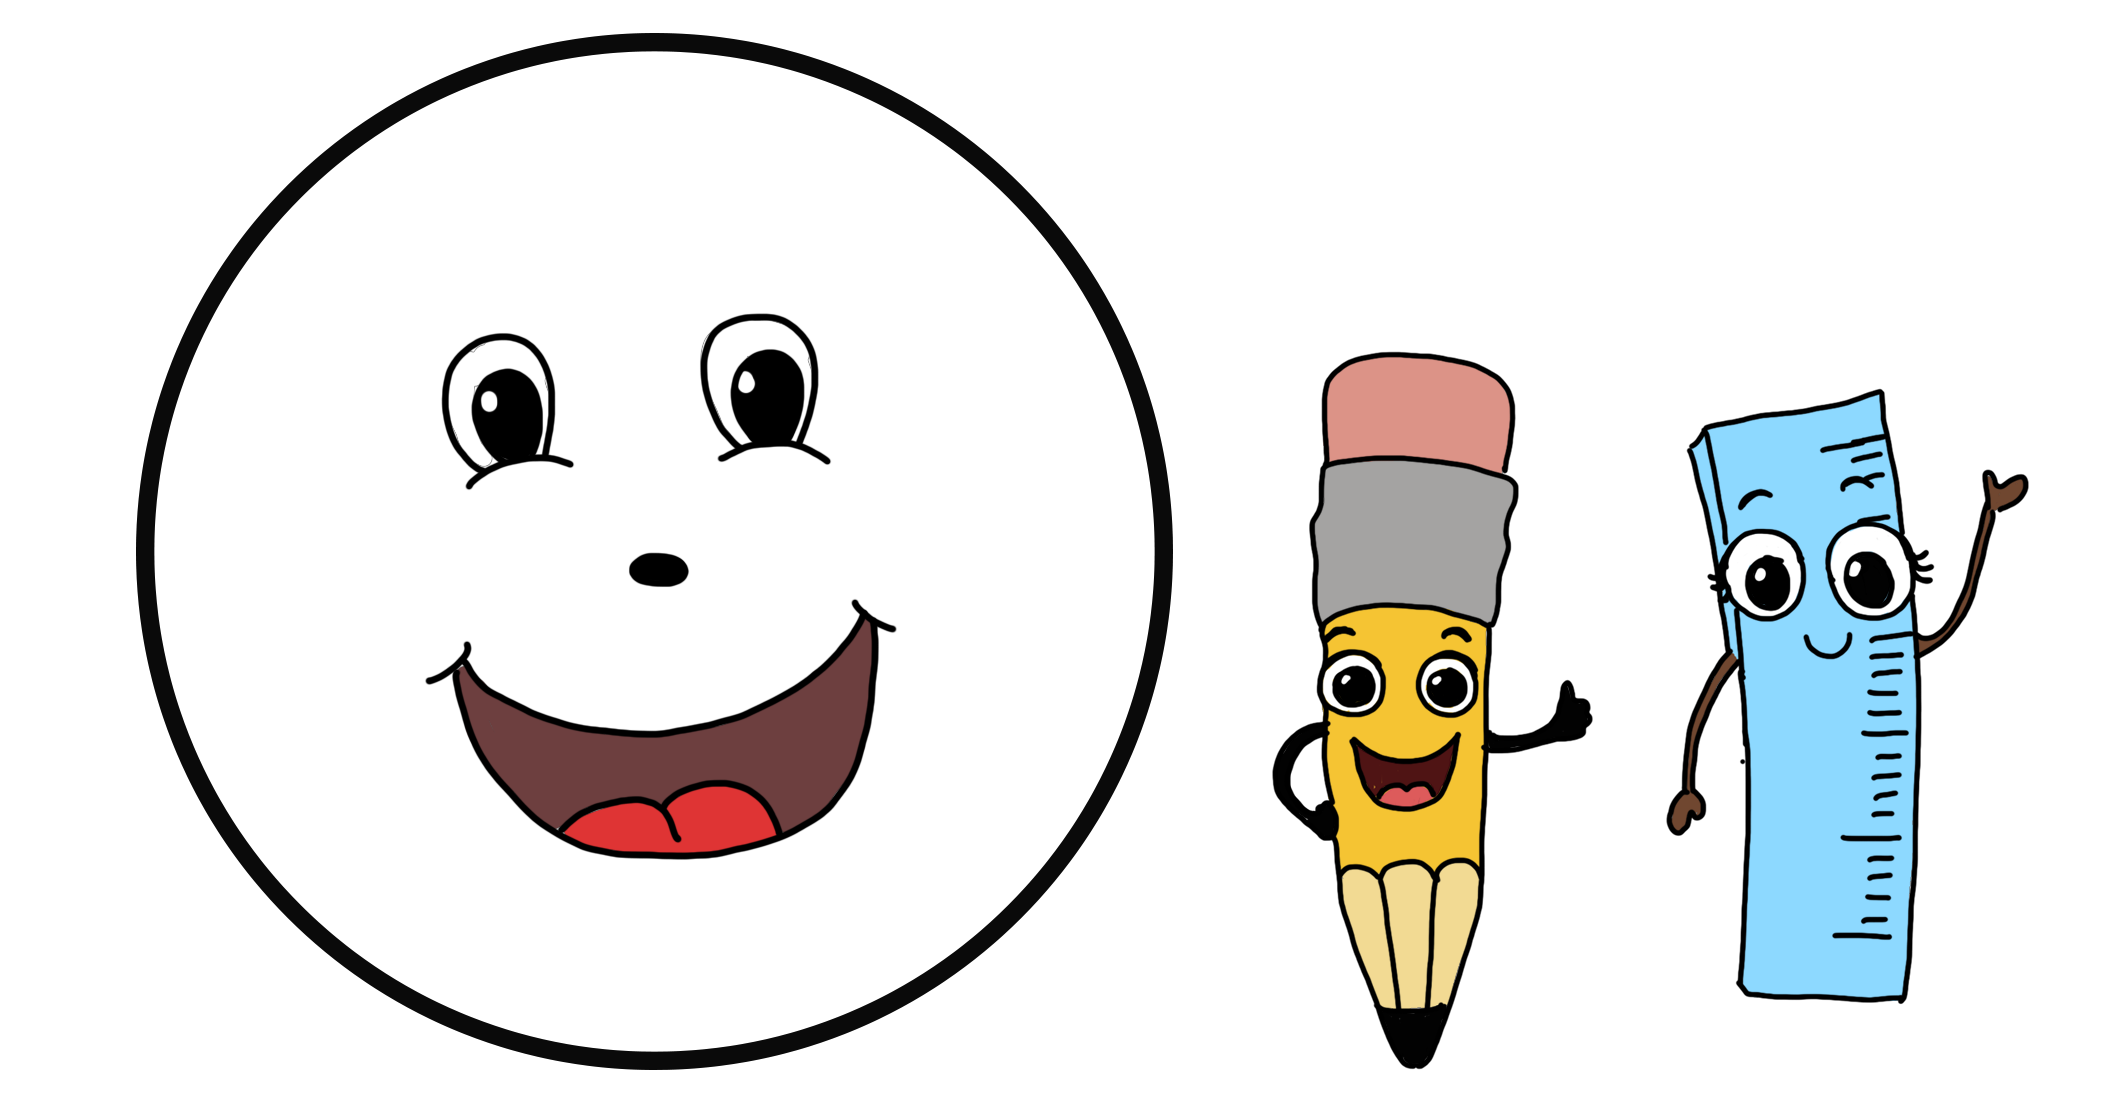
\includegraphics[width=0.7\linewidth]{bai4}
			\vspace*{-15pt}
		\end{figure}
	\textit{Lời giải.} Trong hình dưới đây chỉ ra cách vẽ một đường kính của hình tròn. Các em chỉ cần đặt thước kẻ sao cho ở hai phía của thước hiện ra các phần có độ dài khác nhau. Sau đó nối các điểm như trong hình vẽ, và đường thẳng đi qua $AB$ cũng chứa một đường kính của đường tròn. Các em lại làm tiếp một lần nữa như vậy và rõ ràng giao điểm của hai đường kính sẽ là tâm của hình tròn\linebreak đã cho.
	\begin{figure}[H]
			\centering
			\vspace*{5pt}
			\captionsetup{labelformat= empty, justification=centering}
			\begin{tikzpicture}[scale=0.4,toancuabi]
					\draw [] (0,0) circle (3cm);
					\draw [] (-1.00719,3.55841)-- (-1.007190681933522,-3.6065791726776877);
					\draw [] (-1.0071900697196219,2.8258747607525327)-- (2.583652996516921,-1.5247088881452537);
					\draw [] (2.5836532867476274,1.5247083963427839)-- (-1.0071906076293426,-2.8258745690322558);
					\draw [] (2.5836529350778403,-2.1702415287641776)-- (2.5836533499603247,2.188876204508036);
					\draw [] (-2.005761227573855,3.1877137701678344)-- (7.984604640870016,-0.43236283739412373);
					\draw [] (8.000146076824445,0.43799282872155576)-- (-1.996061700033113,-3.184198481210252);
					
					\draw [fill=white] (-1.0071900697196219,2.8258747607525327) circle (1.6pt);
					\draw [fill=white] (2.5836532867476274,1.5247083963427839) circle (1.6pt);
					\draw [fill=white] (2.583652996516921,-1.5247088881452537) circle (1.6pt);
					\draw [fill=white] (-1.0071906076293426,-2.8258745690322558) circle (1.6pt);
					\draw [fill=white] (6.7914098706510515,-6.46377815560595E-7) circle (1.6pt);
					\draw (6.78454311732612,0.5166504757685513) node {$B$};
					\draw [fill=white] (1.325203480781398,-1.261272915591262E-7) circle (1.6pt);
					\draw (1.2770638218469081,0.607833907812909) node {$A$};
				\end{tikzpicture}
			\vspace*{-10pt}
		\end{figure}
	$\pmb{6.}$ Tất cả các điểm của một đường tròn được tô bằng hai màu: trắng hoặc đỏ. Em hãy chứng tỏ rằng luôn có một tam giác cân có các đỉnh nằm trên đường tròn đã cho sao cho các đỉnh của nó đều được tô bởi cùng một màu.
	\begin{figure}[H]
			\centering
			\vspace*{-10pt}
			\captionsetup{labelformat= empty, justification=centering}
			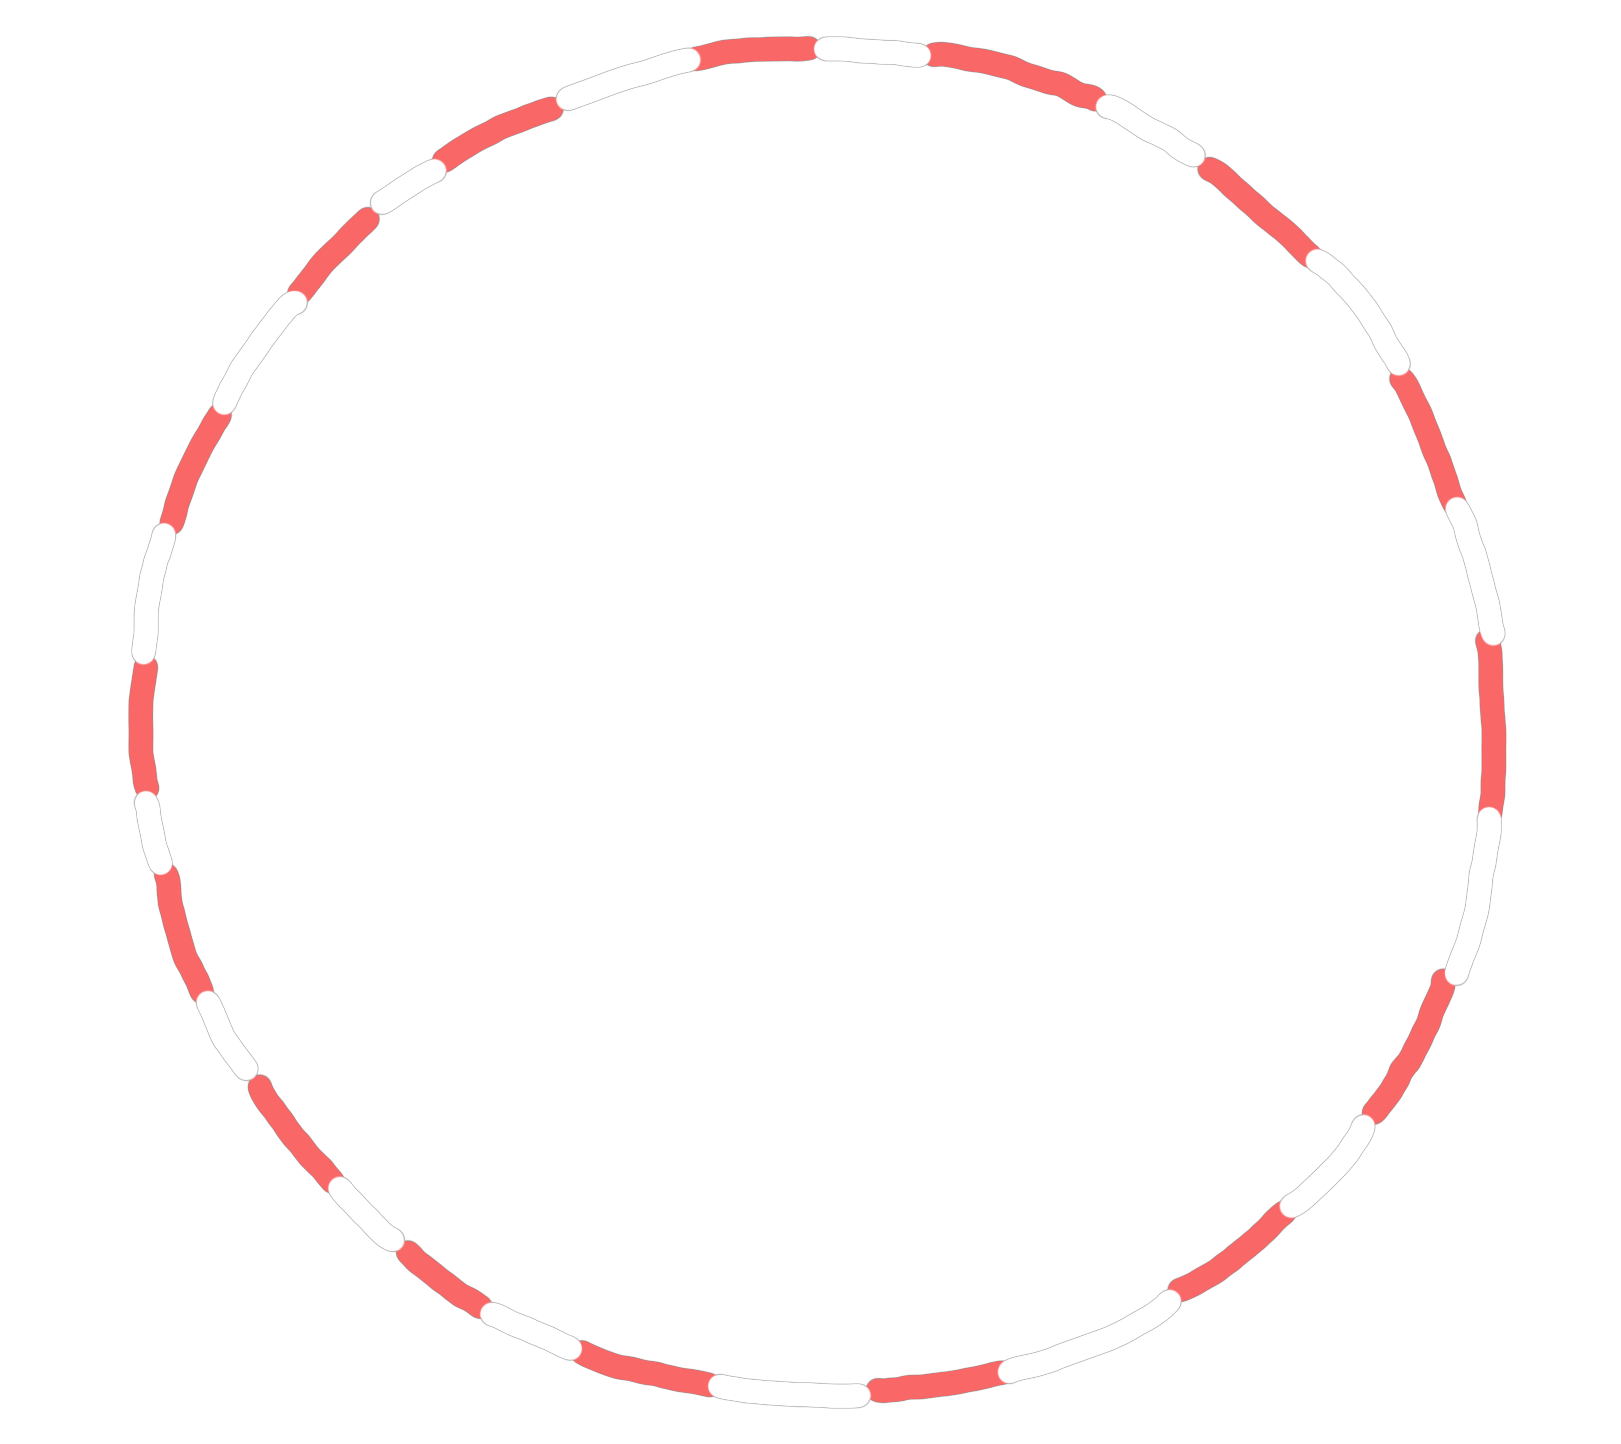
\includegraphics[width=0.6\linewidth]{bai6}
			\vspace*{-5pt}
		\end{figure}
	\textit{Lời giải.} Em  hãy lấy một ngũ giác đều với $5$ đỉnh nằm trên đường tròn đã cho. Bằng nguyên lý Dirichlet dễ thấy phải có ít nhất $3$ đỉnh cùng được tô bởi cùng một màu. Trong mọi cách chọn $3$ đỉnh này, chúng luôn tạo thành một tam giác cân thoả mãn điều kiện của đề bài.
\end{multicols}
%\newpage
%\begingroup
%\thispagestyle{toancuabinone}
%\blfootnote{$^1$\color{toancuabi}Canada.}
%\AddToShipoutPicture*{\put(60,733){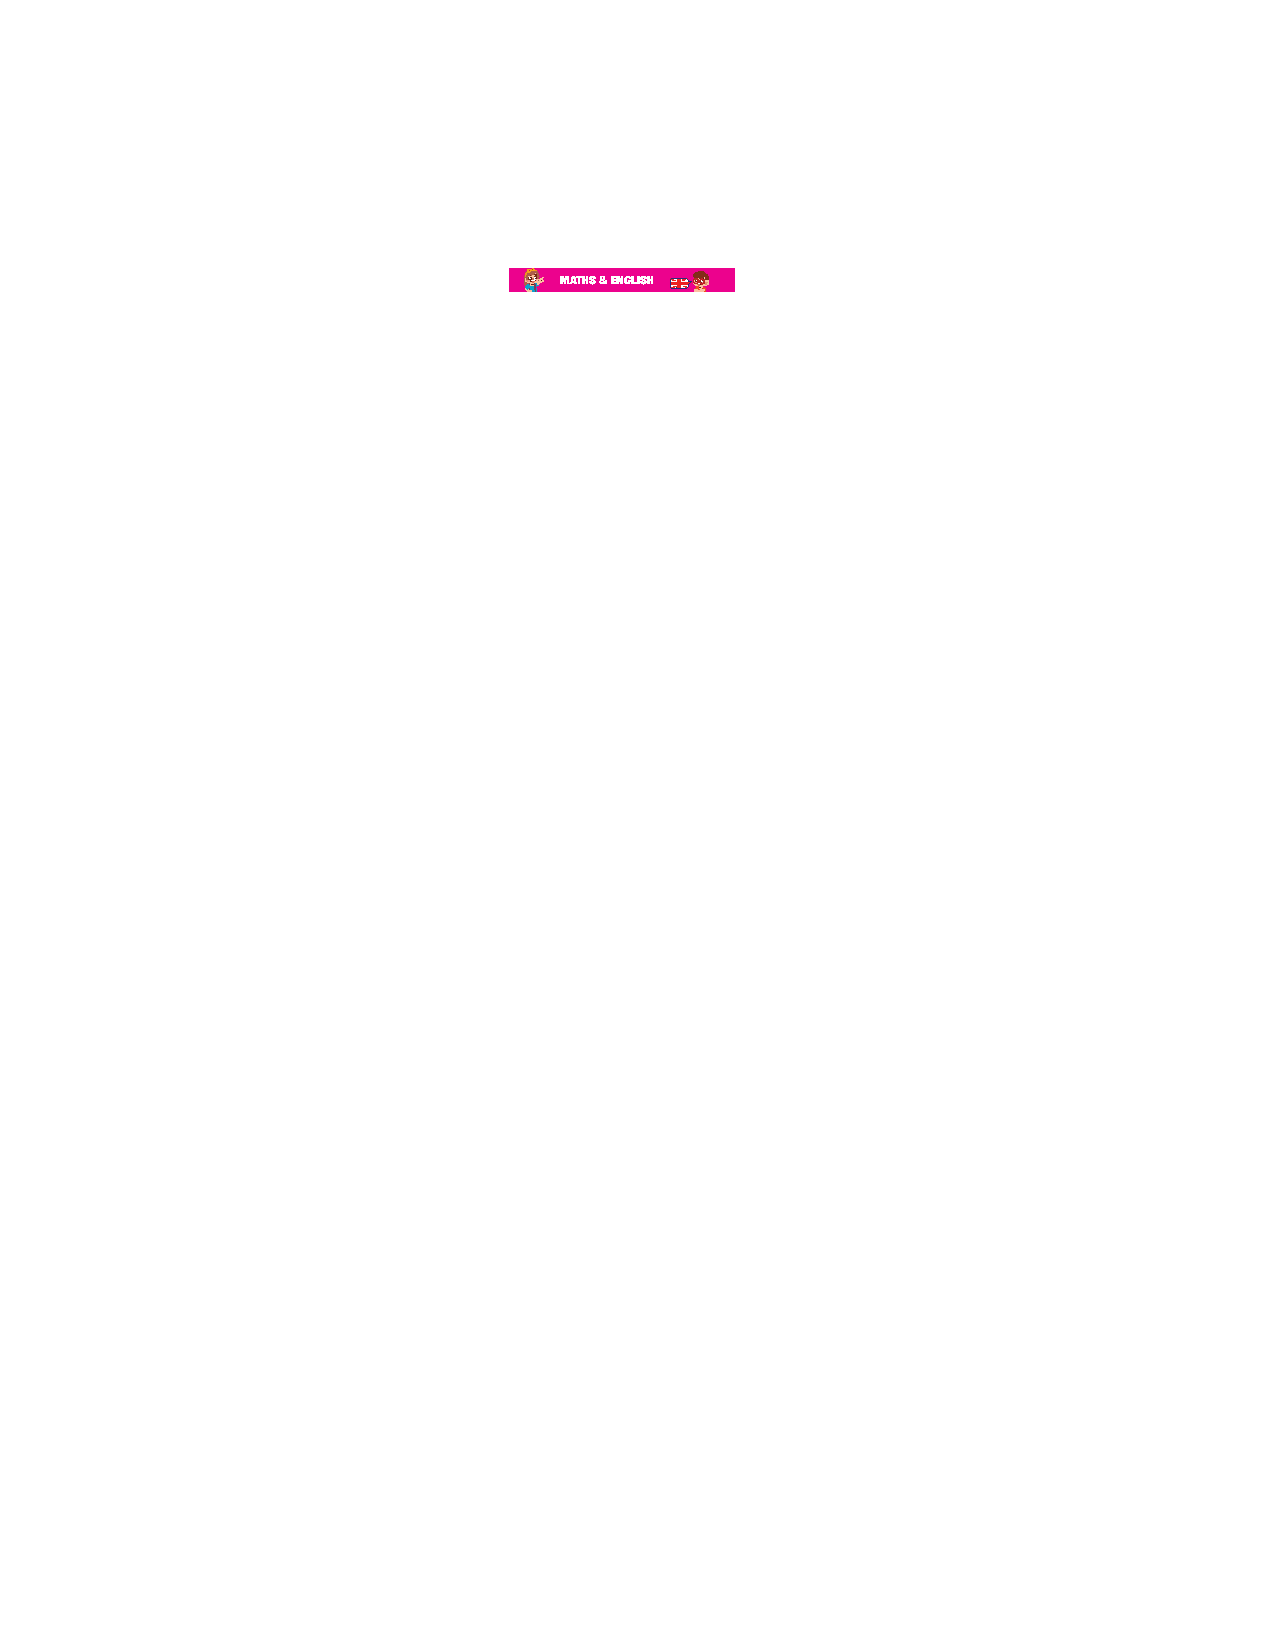
\includegraphics[width=17.2cm]{../mathc.pdf}}}
%%\AddToShipoutPicture*{\put(-2,733){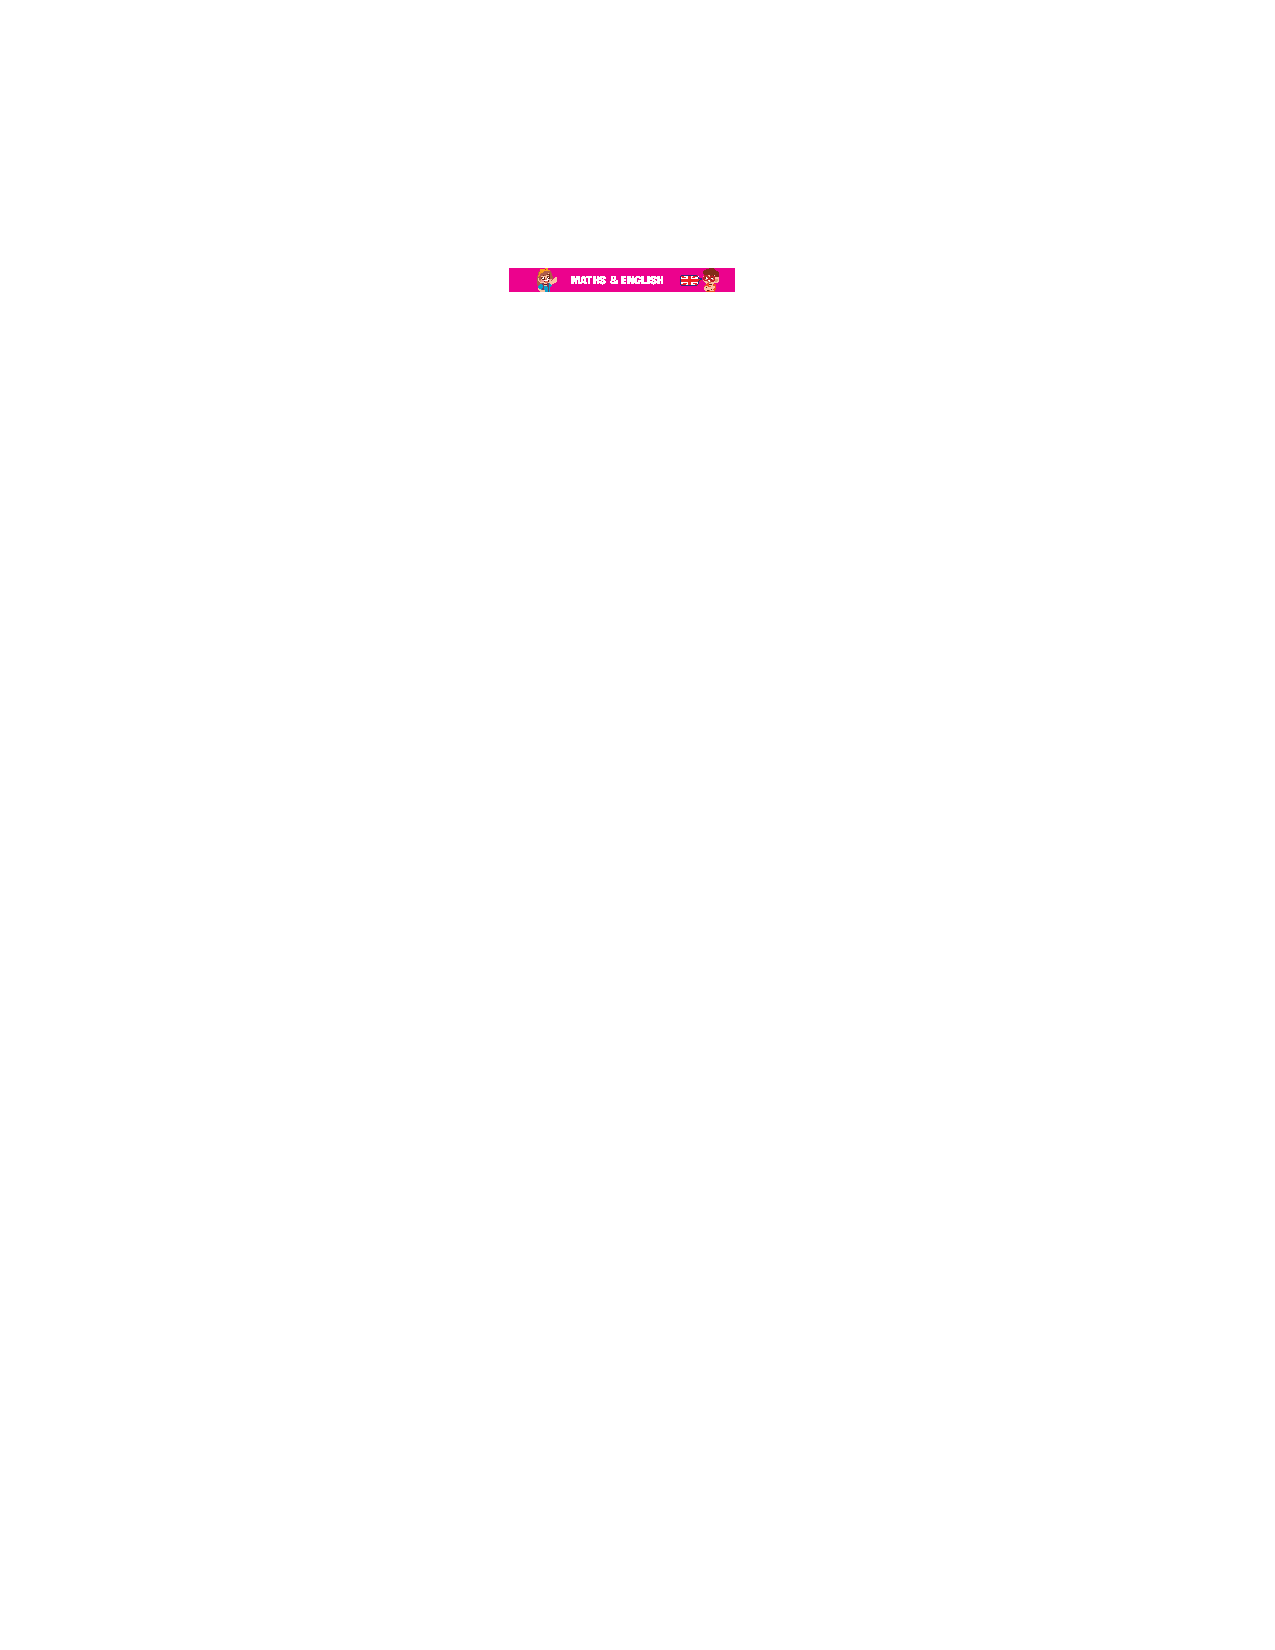
\includegraphics[width=17.2cm]{../mathl.pdf}}} 
%\AddToShipoutPicture*{\put(98,675){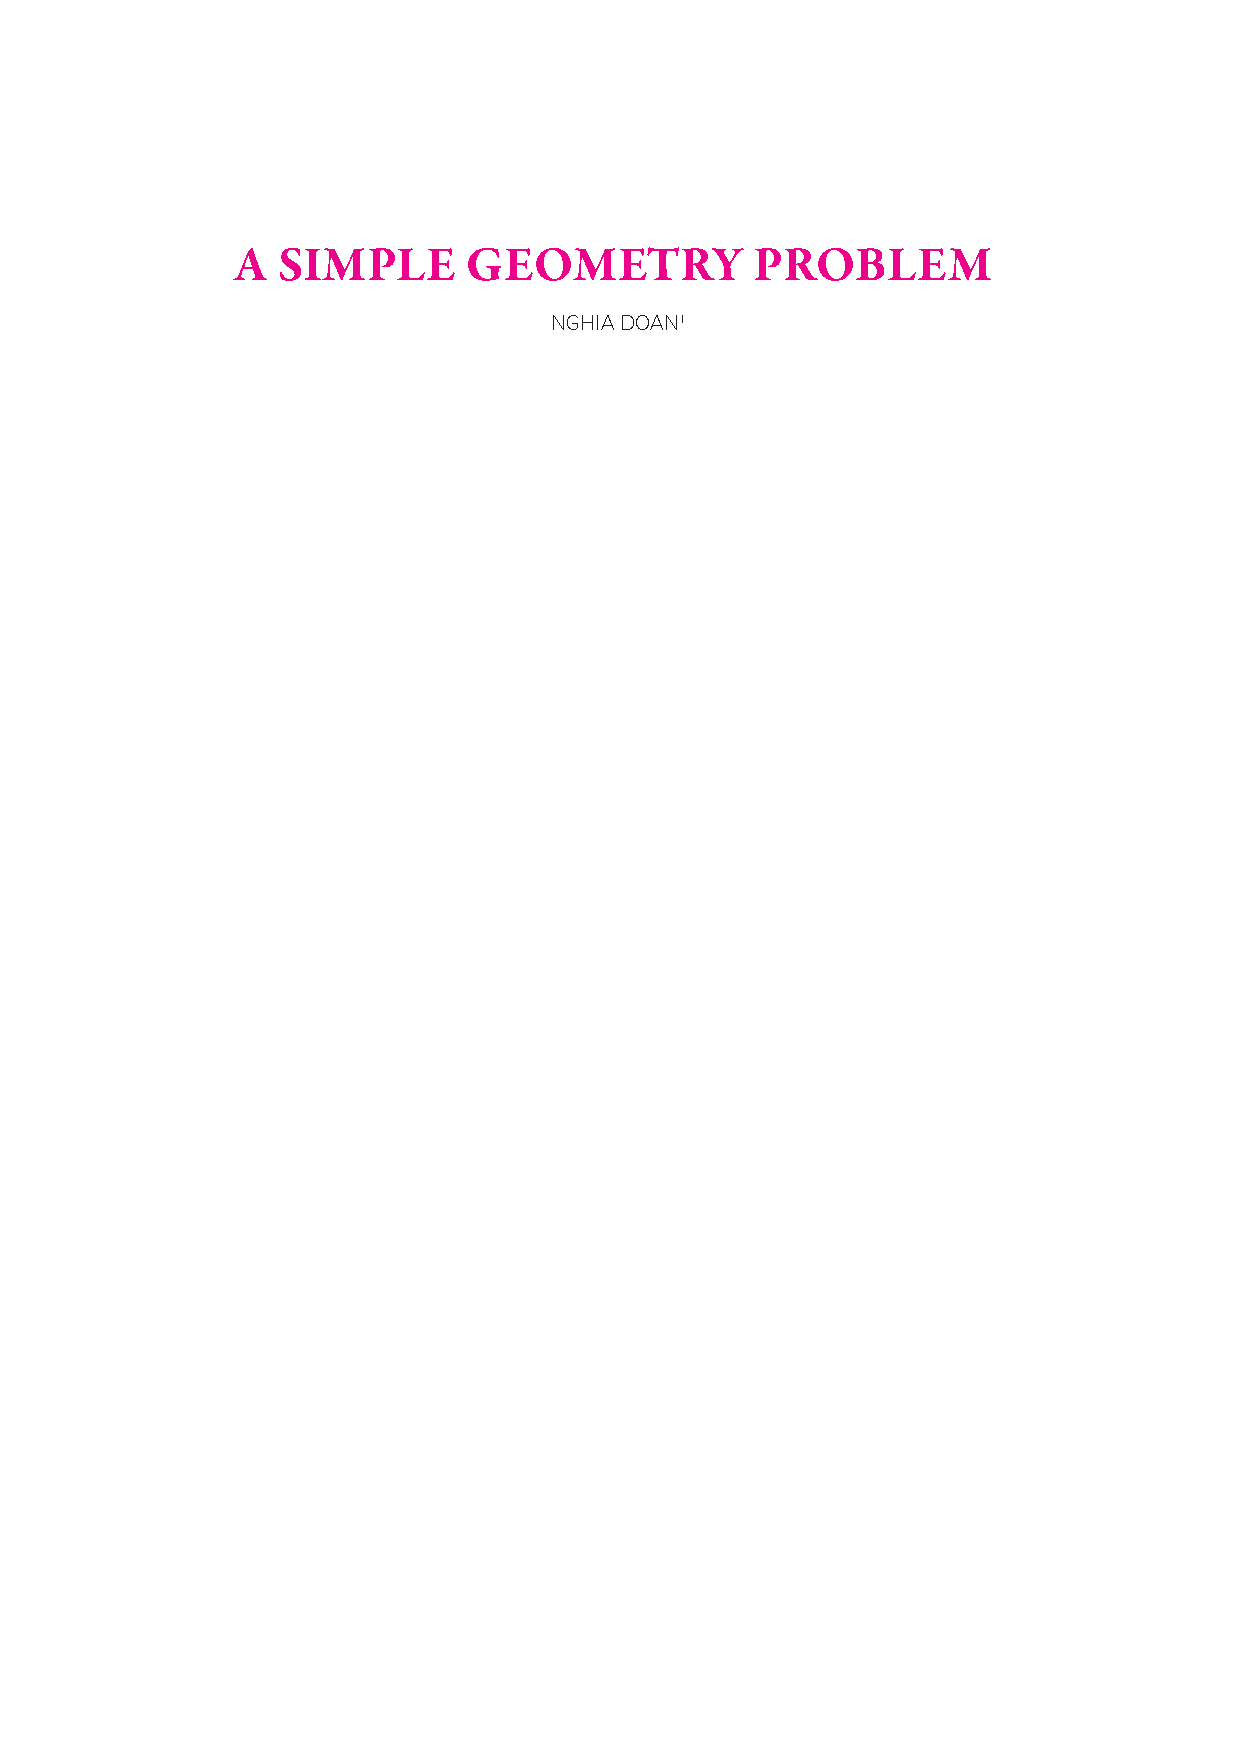
\includegraphics[scale=1]{../tieude3.pdf}}} 
%\centering
%\endgroup
%\graphicspath{{../toancuabi/pic/}}
%\vspace*{35pt}
%
%\begin{multicols}{2}
%	\PIbox{A number is made up of digits.}
%	\vskip 0.1cm
%	\textbf{\color{toancuabi}Divisibility criteria}
%	\vskip 0.1cm
%	We start with some problems using the divisibility criteria for $3, 4,$ or $8$.
%	\vskip 0.1cm
%	\PIbox{\textbf{\color{toancuabi}Problem} $\pmb{1.}$ What is the greatest multiple of $8$ whose digits are all different?}
%	\vskip 0.1cm
%	\textit{Solution.} The greatest multiple of $8$ with different digits has at most ten digits. The {\em divisibility rule} for $8$ states that its last three digits make a number divisible by $8$. If we choose the first seven digits to be $9876543$, then there are digits $0$, $1$ and $2$ left. The greatest multiple of $8$ these three digits can compose is $120$. Thus the desired number is $9876543120$.
%	\vskip 0.15cm
%	\PIbox{\textbf{\color{toancuabi}Problem} $\pmb{2.}$ 
	%		What is the least multiple of $36$ that contains only digits $4$ and $5.$}
%	\vskip 0.1cm
%	\textit{Solution.} Divisibility rule for $9$ states that the sum of digits of the number must be $9, 18, \ldots.$
%	Let's examine  the sum of the digits from the least possible value $9$ and then going up.
%	If the sum is $9,$ then $45$ or $54$ are not divisible by $4,$ so $9=4+5$ is not a possible sum.
%	If the sum is $18,$ the $2-$digit multiple of $4$ can be made from two pairs of $4$ and $5$ is $44.$
%	Thus the number is ${5544}.$
%	\vskip 0.15cm
%	\PIbox{\textbf{\color{toancuabi}Exercise} $\pmb{1.}$ 
	%		Find a $7-$digit number containing only digits $2$ or digits $3$ such that 
	%		there are more of digits $2$ than of digits $3$ and the number is divisible by both $3$ and $4.$}
%	\vskip 0.1cm
%	\textbf{\color{toancuabi}Remainders of  perfect powers}
%	\vskip 0.1cm
%	Now we look at the remainders of a perfect power -- a perfect square, a perfect cube, or a higher power of integer
%	-- when divided by an integer such as $3, 4, 8,9$ or $10,100$ and so on.
%	\vskip 0.1cm
%	\PIbox{\textbf{\color{toancuabi}Problem} $\pmb{3.}$
	%		Is there a $5-$digit perfect square whose sum of digits is $29$?}
%	\vskip 0.1cm
%	\textit{Solution.}
%	A perfect square is divisible by $3$ or has a remainder of $1$ when divided by $3$ (why?).
%	Since the remainder of a number when divided by $3$ is the same as the remainder of its sum of digits when divided by $3,$
%	and $29$ has a remainder of $2$ when divided by $3$ so there is no such number.
%	\vskip 0.1cm
%	\PIbox{\textbf{\color{toancuabi}Problem} $\pmb{4.}$
	%	Find the perfect cube ${n}$ such that all digits of $n$ are $9$ except the unit digit, which is $5.$}
%	\vskip 0.1cm
%	\textit{Solution.}
%	There is no such perfect cube since a perfect cube has a remainder $0, 1,$ or $8$ when divided by $9.$
%	\vskip 0.1cm
%	\PIbox{\textbf{\color{toancuabi}Problem} $\pmb{5.}$
	%		What is the last digit of $\left(... \left((7)^7\right)^7... \right)^{7}$
	%		(there are $1001$ numbers $7)$?}
%	\vskip 0.1cm
%	\textit{Solution.}
%	Testing case by case we have:  $7 \equiv 7 \Mod{10}, 7^7 = (7)(7^2)^3 \equiv -7 \Mod{10}, (7^7)^7 \equiv (-7)^7 \equiv 7 \Mod{10}, \ldots$
%	By Induction Principle, it can be proved that the last digit of the generic expression is $7$ if it has an odd amount of $7,$
%	otherwise it is $3.$ The given one has an odd number of $7,$ so its last digit is ${7.}$  
%	\vskip 0.1cm
%	\PIbox{\textbf{\color{toancuabi}Problem} $\pmb{6.}$
	%		In how many zeros can the number $1^n+2^n+3^n+4^n$ end for ${n}$ positive integer?}
%	\vskip 0.1cm
%	\textit{Solution.}
%	For $n=1,$ and $2,$ the sum ends in one and two zeros.
%	Now, for all $n \ge 3,$ $2^n, 4^n$ are divisible by $8,$
%	and $1^n + 3^n$ congruent to $2$ or $4$ modulo $8$.
%	Thus, the sum cannot end in three or more zeros.
%	\vskip 0.1cm
%	\PIbox{\textbf{\color{toancuabi}Exercise} $\pmb{2.}$
	%		\label{exercise:twelf}
	%		Find the last five digits of $5^{1981}.$}
%	\vskip 0.1cm
%	\PIbox{\textbf{\color{toancuabi}Exercise} $\pmb{3.}$
	%		Find ${n} > 3$ such that the $(n+1)$--digit binary number $\overline{10\ldots01_2}$ is a perfect power of $3.$}
%	\vskip 0.1cm
%	\textbf{\color{toancuabi}Relations between digits of a number}
%	\vskip 0.1cm
%	\PIbox{\textbf{\color{toancuabi}Problem} $\pmb{7.}$
	%		Digits ${a}$, ${b}$, and ${c}$ are used to form $3-$digit numbers $\overline{abc}, \overline{bca},$ and $\overline{cab}.$
	%		The sum of these numbers is $1332,$ find $a+b+c.$}
%	\vskip 0.1cm
%	\textit{Solution.}
%	$\overline{abc} = 100a + 10b + c,$ similarly with others. Their sum is $111(a+b+c)=1332,$ $a+b+c=12.$
%	\vskip 0.1cm
%	\PIbox{\textbf{\color{toancuabi}Problem} $\pmb{8.}$
	%		Find all $4-$digit number ${n}$ whose sum of digits is $2010-n.$}
%	\vskip 0.1cm
%	\textit{Solution.}
%	Let $n=\overline{abcd}.$ Then $1001a+101b+11c+2d=2010.$ If $a=1,$ then $b=9,$ so $11c+2d=100,$ so $c=8,d=2.$
%	If $a=2,$ then $b=c=0,d=4.$ The solutions are ${1982,\ 2004}.$
%	\vskip 0.1cm
%	\PIbox{\textbf{\color{toancuabi}Exercise} $\pmb{4.}$
	%		Find a potitive integer ${a}$ such that $(1+2+\ldots + a)- 1000a$ is a $3-$digit number. }
%	\vskip 0.1cm
%	\textbf{\color{toancuabi}Hints to the exercises}
%	\vskip 0.1cm
%	\textbf{\color{toancuabi}Exercise} $\pmb{1.}$ First find the last two digits based on divisibility rule for $4.$
%	Then find the number of digits $2$ in the first five digits.
%	\vskip 0.1cm
%	\textbf{\color{toancuabi}Exercise} $\pmb{2.}$
%	Let $\overline{10\ldots01_2} = 2^n + 1 = 3^m.$ There are two cases: $m$ is odd or even. 
%	\vskip 0.1cm
%	\textbf{\color{toancuabi}Exercise} $\pmb{3.}$
%	There are two cases, $a < 1999$ and $a \ge 2000.$
%	\vskip 0.1cm
%	\textbf{\color{toancuabi}Exercise} $\pmb{4.}$	Find the last $5$ digits of $5^{1981} - 5^5 = 5^5(5^{1976}-1).$
%	\vskip 0.1cm
%	\PIbox{
	%	{\centerline{\textbf{\color{toancuabi}New Words}}}
	%	\vskip 0.1cm
	%	{\color{toancuabi}Binary (adj):} nhị phân 
	%	\vskip 0.1cm
	%	{\color{toancuabi}Criteria (n,pl):} dấu hiệu
	%	\vskip 0.1cm
	%	{\color{toancuabi}Cube (n):} lập phương
	%	\vskip 0.1cm
	%	{\color{toancuabi}Digit (n):} chữ số 
	%	\vskip 0.1cm
	%	{\color{toancuabi}Divisibility (n):} tính chia hết 
	%	\vskip 0.1cm
	%	{\color{toancuabi}Multiple (n):} bội số
	%	\vskip 0.1cm
	%	{\color{toancuabi}Perfect (adj):} hoàn thiện 
	%	\vskip 0.1cm
	%	{\color{toancuabi}Perfect square (n):} số chính phương
	%	\vskip 0.1cm
	%	{\color{toancuabi}Power (n):} lũy thừa 
	%	\vskip 0.1cm
	%	{\color{toancuabi}Relation (n):} hệ thức 
	%	\vskip 0.1cm
	%	{\color{toancuabi}Remainder (n):} số dư (trong phép chia)
	%	}
%\end{multicols}